\documentclass[11pt,a4paper]{article}
\usepackage[margin=1.9cm, top=2.1cm, bottom=2.0cm]{geometry}
\usepackage[T1]{fontenc}
\usepackage{lmodern}
\usepackage{amsmath,amssymb}
\usepackage{enumitem,booktabs,array,tabularx,multirow}
\usepackage[normalem]{ulem}
\usepackage{adjustbox}
\usepackage{xcolor}
\usepackage{fancyhdr,lastpage}
\usepackage[most]{tcolorbox}
\usepackage{tikz}
\usetikzlibrary{shapes.geometric,arrows.meta,positioning,calc}
\usepackage[hidelinks]{hyperref}
\setlength{\parindent}{0pt}
\setlength{\parskip}{4pt}
\renewcommand{\arraystretch}{1.25}
\emergencystretch=2em
\pagestyle{fancy}\fancyhf{}
\lhead{\small\textit{Course: CS420 -- Artificial Intelligence}}
\rhead{\small Practice Test 2 -- Solution}
\cfoot{\small Page \thepage\ of \pageref{LastPage}}
\renewcommand{\headrulewidth}{0.4pt}
% empty answer box (exam) / filled box (solution)
\newtcolorbox{ansbox}[1][]{enhanced, breakable, colback=white, colframe=black!55, boxrule=0.5pt, arc=0pt,
  left=5pt, right=5pt, top=3pt, bottom=3pt, before skip=3pt, after skip=6pt, #1}
\newtcolorbox{solbox}{enhanced, breakable, colback=blue!2!white, colframe=blue!50!black, boxrule=0.6pt, arc=0pt,
  left=6pt, right=6pt, top=4pt, bottom=4pt, before skip=3pt, after skip=8pt,
  fontupper=\color{black}}
\newcommand{\question}[1]{\par\medskip\noindent\textbf{Question #1.}\ }
\newcommand{\subq}[1]{\par\smallskip\noindent\textbf{#1}\ }
\newcommand{\T}{\textbf{\textcolor{green!45!black}{TRUE}}}
\newcommand{\F}{\textbf{\textcolor{red!70!black}{FALSE}}}

\tikzset{
  maxn/.style={draw, thick, regular polygon, regular polygon sides=3, minimum size=10.5mm, inner sep=0pt, font=\small},
  minn/.style={maxn, shape border rotate=180},
  chn/.style={draw, thick, circle, minimum size=9.5mm, inner sep=0pt, font=\small},
  leafn/.style={draw, rectangle, minimum width=5.5mm, minimum height=5.5mm, inner sep=1pt, font=\small},
  gone/.style={draw=black!25, text=black!35},
  cut/.style={red!80!black, very thick, dashed},
  sol/.style={text=blue!70!black, font=\small\bfseries},
}

\begin{document}


{\large\textbf{\textit{Course: CS420 -- Artificial Intelligence}}}\par
{\textbf{\textit{Midterm examination review -- Lectures 0 to 3}}}\par
\begin{center}{\Large\bfseries PRACTICE MIDTERM EXAMINATION -- TEST 2\\[2pt]\textcolor{blue!55!black}{SOLUTION}}\\[3pt]
{\small Duration: 120 minutes \quad$\cdot$\quad Closed book \quad$\cdot$\quad Calculator allowed}\end{center}
\noindent\rule{\linewidth}{0.6pt}

{\small\textit{Unless a question says otherwise, ties are broken in alphabetical order (left-to-right in trees), and successors are generated in alphabetical order.}}\par
\question{1}\textit{Farmer, wolf, goat and cabbage.} A farmer must take a wolf, a goat and a cabbage across a river. The boat holds the farmer and at most one of the three items, and only the farmer can row. Left unattended (without the farmer), the wolf eats the goat and the goat eats the cabbage.
\subq{(a)}Consider a state as a tuple of values. Which values should be included in the tuple?
\begin{solbox}
$(F, W, G, C)$: the bank (L or R) on which the farmer, the wolf, the goat and the cabbage are. (The boat is always with the farmer.)
\end{solbox}
\subq{(b)}Define the initial state and the goal state.
\begin{solbox}
Initial $(L,L,L,L)$; goal $(R,R,R,R)$.
\end{solbox}
\subq{(c)}Define the action function.
\begin{solbox}
The farmer crosses alone or with one item that is on \emph{his} bank: Cross, CrossW, CrossG, CrossC. An action is legal only if the result does not leave W with G, or G with C, on the bank without the farmer.
\end{solbox}
\subq{(d)}What is the action cost?
\begin{solbox}
1 per crossing.
\end{solbox}
\subq{(e)}What is the maximum number of states (including illegal ones)? How many states are legal, and how many are reachable? Give a shortest solution.
\begin{solbox}
$2^4=\mathbf{16}$ tuples, \textbf{10} legal, \textbf{10} reachable. Shortest solution (7 crossings): LLLL $\to$ RLRL $\to$ LLRL $\to$ RRRL $\to$ LRLL $\to$ RRLR $\to$ LRLR $\to$ RRRR.
\end{solbox}
\question{2}Consider the \emph{directed} graph below; $S$ is the initial state and $G$ the goal state. \begin{center}
\begin{adjustbox}{max width=\linewidth}
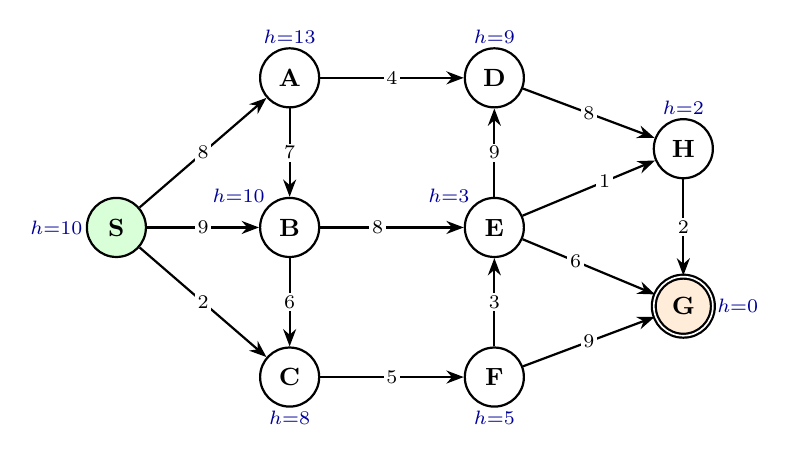
\begin{tikzpicture}[scale=1.0, every node/.style={transform shape}, gn/.style={draw, thick, circle, minimum size=7.5mm, inner sep=0pt, font=\small\bfseries}, ec/.style={font=\scriptsize, fill=white, inner sep=1pt}]
\node[gn, fill=green!15, label={[font=\scriptsize, text=blue!60!black, inner sep=1pt]left:$h{=}10$}] (S) at (0.00,0.00) {S};
\node[gn, label={[font=\scriptsize, text=blue!60!black, inner sep=1pt]above:$h{=}13$}] (A) at (2.20,1.90) {A};
\node[gn, label={[font=\scriptsize, text=blue!60!black, inner sep=1pt]above left:$h{=}10$}] (B) at (2.20,0.00) {B};
\node[gn, label={[font=\scriptsize, text=blue!60!black, inner sep=1pt]below:$h{=}8$}] (C) at (2.20,-1.90) {C};
\node[gn, label={[font=\scriptsize, text=blue!60!black, inner sep=1pt]above:$h{=}9$}] (D) at (4.80,1.90) {D};
\node[gn, label={[font=\scriptsize, text=blue!60!black, inner sep=1pt]above left:$h{=}3$}] (E) at (4.80,0.00) {E};
\node[gn, label={[font=\scriptsize, text=blue!60!black, inner sep=1pt]below:$h{=}5$}] (F) at (4.80,-1.90) {F};
\node[gn, label={[font=\scriptsize, text=blue!60!black, inner sep=1pt]above:$h{=}2$}] (H) at (7.20,1.00) {H};
\node[gn, double, fill=orange!15, label={[font=\scriptsize, text=blue!60!black, inner sep=1pt]right:$h{=}0$}] (G) at (7.20,-1.00) {G};
\draw[thick,-{Stealth[length=2.2mm]}] (S) to[] node[ec, midway]{8} (A);
\draw[thick,-{Stealth[length=2.2mm]}] (S) to[] node[ec, midway]{9} (B);
\draw[thick,-{Stealth[length=2.2mm]}] (S) to[] node[ec, midway]{2} (C);
\draw[thick,-{Stealth[length=2.2mm]}] (A) to[] node[ec, midway]{4} (D);
\draw[thick,-{Stealth[length=2.2mm]}] (A) to[] node[ec, midway]{7} (B);
\draw[thick,-{Stealth[length=2.2mm]}] (B) to[] node[ec, pos=0.4]{8} (E);
\draw[thick,-{Stealth[length=2.2mm]}] (C) to[] node[ec, midway]{5} (F);
\draw[thick,-{Stealth[length=2.2mm]}] (B) to[] node[ec, midway]{6} (C);
\draw[thick,-{Stealth[length=2.2mm]}] (D) to[] node[ec, midway]{8} (H);
\draw[thick,-{Stealth[length=2.2mm]}] (E) to[] node[ec, midway]{9} (D);
\draw[thick,-{Stealth[length=2.2mm]}] (E) to[] node[ec, pos=0.4]{6} (G);
\draw[thick,-{Stealth[length=2.2mm]}] (F) to[] node[ec, midway]{3} (E);
\draw[thick,-{Stealth[length=2.2mm]}] (F) to[] node[ec, midway]{9} (G);
\draw[thick,-{Stealth[length=2.2mm]}] (H) to[] node[ec, midway]{2} (G);
\draw[thick,-{Stealth[length=2.2mm]}] (E) to[] node[ec, pos=0.62]{1} (H);
\end{tikzpicture}
\end{adjustbox}
\end{center}For each search strategy, (a) list, in order, the states \textbf{expanded}, (b) give the path found and (c) give the final content of the frontier (a state is expanded when it is removed from the frontier). Conventions: BFS, DFS and greedy best-first search test a state for the goal when it is \emph{generated} (so the goal is not expanded); UCS and A* test it when it is \emph{removed} from the frontier (graph search; a cheaper path to a frontier state replaces its entry). DFS avoids loops by remembering the states on the current path only. The path returned will not be accepted if the list of expanded states is wrong.

\begin{solbox}
\begin{center}\small\begin{tabularx}{\linewidth}{|>{\raggedright}p{2.6cm}|>{\raggedright}X|>{\raggedright}p{3.6cm}|>{\raggedright\arraybackslash}p{2.6cm}|}\hline
\textbf{Algorithm} & \textbf{List of expanded states} & \textbf{Path returned} & \textbf{Final frontier}\\ \hline
Breadth-first search & \textcolor{blue!60!black}{S A B C D E} & \textcolor{blue!60!black}{S B E G} (cost 23) & \textcolor{blue!60!black}{$\{$ F, H $\}$}\\ \hline
Uniform-cost search & \textcolor{blue!60!black}{S C F A B E H D G} & \textcolor{blue!60!black}{S C F E H G} (cost 13) & \textcolor{blue!60!black}{$\{\ \}$}\\ \hline
Depth-first search & \textcolor{blue!60!black}{S A B C F} & \textcolor{blue!60!black}{S A B C F G} (cost 35) & \textcolor{blue!60!black}{(not asked)}\\ \hline
Greedy best-first search & \textcolor{blue!60!black}{S C F} & \textcolor{blue!60!black}{S C F G} (cost 16) & \textcolor{blue!60!black}{$\{$ E, B, A $\}$}\\ \hline
Graph-search A* & \textcolor{blue!60!black}{S C F E H G} & \textcolor{blue!60!black}{S C F E H G} (cost 13) & \textcolor{blue!60!black}{$\{$ B, A, D $\}$}\\ \hline
\end{tabularx}\end{center}\textbf{BFS} (queue after each expansion):\begin{center}\small\begin{tabularx}{\linewidth}{c c >{\raggedright\arraybackslash}X}\toprule
Step & Expanded & Queue (front $\rightarrow$ back) after the expansion \\ \midrule
1 & S & A, B, C \\
2 & A & B, C, D \\
3 & B & C, D, E \\
4 & C & D, E, F \\
5 & D & E, F, H \\
6 & E & generates goal \textbf{G} $\Rightarrow$ stop; frontier: F, H \\
\bottomrule\end{tabularx}\end{center}\textbf{DFS} (stack after each expansion):\begin{center}\small\begin{tabularx}{\linewidth}{c c >{\raggedright\arraybackslash}X}\toprule
Step & Expanded & Stack (top $\rightarrow$ bottom) after the expansion \\ \midrule
1 & S & A, B, C \\
2 & A & B, D, B, C \\
3 & B & C, E, D, B, C \\
4 & C & F, E, D, B, C \\
5 & F & generates goal \textbf{G} $\Rightarrow$ stop; frontier: E, D, B, C \\
\bottomrule\end{tabularx}\end{center}\textbf{UCS:}\begin{center}\small\begin{tabularx}{\linewidth}{c l >{\raggedright\arraybackslash}X}\toprule
Step & Expanded & Frontier after the expansion, in priority order (subscript $=g(n)$) \\ \midrule
1 & S$_{0}$ & C$_{2}$, A$_{8}$, B$_{9}$ \\
2 & C$_{2}$ & F$_{7}$, A$_{8}$, B$_{9}$ \\
3 & F$_{7}$ & A$_{8}$, B$_{9}$, E$_{10}$, G$_{16}$ \\
4 & A$_{8}$ & B$_{9}$, E$_{10}$, D$_{12}$, G$_{16}$ \\
5 & B$_{9}$ & E$_{10}$, D$_{12}$, G$_{16}$ \\
6 & E$_{10}$ & H$_{11}$, D$_{12}$, G$_{16}$ \\
7 & H$_{11}$ & D$_{12}$, G$_{13}$ \\
8 & D$_{12}$ & G$_{13}$ \\
9 & G$_{13}$ & \textit{goal removed from the frontier -- stop} \\
\bottomrule\end{tabularx}\end{center}\textbf{Greedy best-first:}\begin{center}\small\begin{tabularx}{\linewidth}{c l >{\raggedright\arraybackslash}X}\toprule
Step & Expanded & Frontier after the expansion, in priority order (subscript $=h(n)$) \\ \midrule
1 & S$_{10}$ & C$_{8}$, B$_{10}$, A$_{13}$ \\
2 & C$_{8}$ & F$_{5}$, B$_{10}$, A$_{13}$ \\
3 & F$_{5}$ & generates goal \textbf{G} $\Rightarrow$ stop; frontier: E$_{3}$, B$_{10}$, A$_{13}$ \\
\bottomrule\end{tabularx}\end{center}\textbf{A*:}\begin{center}\small\begin{tabularx}{\linewidth}{c l >{\raggedright\arraybackslash}X}\toprule
Step & Expanded & Frontier after the expansion, in priority order (subscript $=g+h=f$) \\ \midrule
1 & S$_{0+10=10}$ & C$_{2+8=10}$, B$_{9+10=19}$, A$_{8+13=21}$ \\
2 & C$_{2+8=10}$ & F$_{7+5=12}$, B$_{9+10=19}$, A$_{8+13=21}$ \\
3 & F$_{7+5=12}$ & E$_{10+3=13}$, G$_{16+0=16}$, B$_{9+10=19}$, A$_{8+13=21}$ \\
4 & E$_{10+3=13}$ & H$_{11+2=13}$, G$_{16+0=16}$, B$_{9+10=19}$, A$_{8+13=21}$, D$_{19+9=28}$ \\
5 & H$_{11+2=13}$ & G$_{13+0=13}$, B$_{9+10=19}$, A$_{8+13=21}$, D$_{19+9=28}$ \\
6 & G$_{13+0=13}$ & \textit{goal removed from the frontier -- stop} \\
\bottomrule\end{tabularx}\end{center}
\end{solbox}
\subq{(d)}Is $h$ admissible? Is it consistent? Justify (only the direction of each edge matters).
\begin{solbox}
$h^*$: S$=13$, A$=14$, B$=11$, C$=11$, D$=10$, E$=3$, F$=6$, H$=2$, G$=0$. $h\le h^*$ everywhere $\Rightarrow$ admissible; $h(u)\le c(u,v)+h(v)$ for every directed edge $u\to v$ $\Rightarrow$ consistent.
\end{solbox}
\subq{(e)}UCS and A* return the same path. Why does A* expand fewer states?
\begin{solbox}
Both are optimal here (cost 13). A* never expands a state with $f(n)>C^*$: $A$ ($f=8+13=21$) and $B$ ($f=9+10=19$) are never expanded, so A* expands 6 states versus 9 for UCS.
\end{solbox}
\question{3}\textit{4-bishops.} Consider the 4-bishops problem: every state has 4 bishops on a $4\times4$ board, one in each column. A bishop attacks along the diagonals (count attacking pairs regardless of pieces in between).\begin{center}
\begin{adjustbox}{max width=\linewidth}
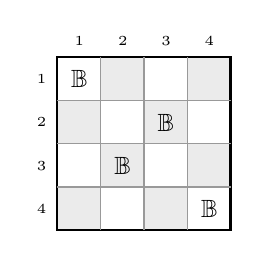
\begin{tikzpicture}
\fill[white] (0.00,0.00) rectangle +(0.55,-0.55);
\fill[black!8] (0.00,-0.55) rectangle +(0.55,-0.55);
\fill[white] (0.00,-1.10) rectangle +(0.55,-0.55);
\fill[black!8] (0.00,-1.65) rectangle +(0.55,-0.55);
\fill[black!8] (0.55,0.00) rectangle +(0.55,-0.55);
\fill[white] (0.55,-0.55) rectangle +(0.55,-0.55);
\fill[black!8] (0.55,-1.10) rectangle +(0.55,-0.55);
\fill[white] (0.55,-1.65) rectangle +(0.55,-0.55);
\fill[white] (1.10,0.00) rectangle +(0.55,-0.55);
\fill[black!8] (1.10,-0.55) rectangle +(0.55,-0.55);
\fill[white] (1.10,-1.10) rectangle +(0.55,-0.55);
\fill[black!8] (1.10,-1.65) rectangle +(0.55,-0.55);
\fill[black!8] (1.65,0.00) rectangle +(0.55,-0.55);
\fill[white] (1.65,-0.55) rectangle +(0.55,-0.55);
\fill[black!8] (1.65,-1.10) rectangle +(0.55,-0.55);
\fill[white] (1.65,-1.65) rectangle +(0.55,-0.55);
\draw[thick] (0,0) rectangle (2.20,-2.20);
\draw[black!40] (0.55,0) -- (0.55,-2.20);
\draw[black!40] (0,-0.55) -- (2.20,-0.55);
\draw[black!40] (1.10,0) -- (1.10,-2.20);
\draw[black!40] (0,-1.10) -- (2.20,-1.10);
\draw[black!40] (1.65,0) -- (1.65,-2.20);
\draw[black!40] (0,-1.65) -- (2.20,-1.65);
\node[font=\small\bfseries] at (0.28,-0.28) {$\mathbb{B}$};
\node[font=\small\bfseries] at (0.83,-1.38) {$\mathbb{B}$};
\node[font=\small\bfseries] at (1.38,-0.83) {$\mathbb{B}$};
\node[font=\small\bfseries] at (1.93,-1.93) {$\mathbb{B}$};
\node[font=\tiny] at (0.28,0.20) {1};
\node[font=\tiny] at (0.83,0.20) {2};
\node[font=\tiny] at (1.38,0.20) {3};
\node[font=\tiny] at (1.93,0.20) {4};
\node[font=\tiny] at (-0.20,-0.28) {1};
\node[font=\tiny] at (-0.20,-0.83) {2};
\node[font=\tiny] at (-0.20,-1.38) {3};
\node[font=\tiny] at (-0.20,-1.93) {4};
\end{tikzpicture}
\end{adjustbox}
\end{center}
\subq{(a)}What is the total number of states in the state space? Explain.
\begin{solbox}
$4^4=\mathbf{256}$: each of the 4 bishops can be in any of the 4 rows of its column.
\end{solbox}
\subq{(b)}Each step moves one bishop within its own column. How many successors does a state have? Explain.
\begin{solbox}
$4\times3=\mathbf{12}$: choose the bishop (4 ways) and one of the 3 other rows of its column.
\end{solbox}
\subq{(c)}A state is written as 4 digits giving the row of the bishop in columns 1--4 (the board above is 1324). Let $n_b$ be the number of attacking pairs of bishops of state $n$. Define a fitness function Fit$(n)$ to be maximised by the genetic algorithm.
\begin{solbox}
Fit$(n)=\binom42-n_b=6-n_b$ (the number of non-attacking pairs); the goal has Fit $=6$.
\end{solbox}
\subq{(d)}The current generation is $S_1=1324$, $S_2=2143$, $S_3=3412$, $S_4=4132$. Compute Fit$(n)$ and the probability that each state is chosen in the roulette-wheel selection step. Then cross $S_1$ with $S_4$ after the 2nd digit and give the two children with their fitness.
\begin{solbox}
\begin{center}\begin{tabular}{|l|c|c|c|c|}\hline State $n$ & $S_1=1324$ & $S_2=2143$ & $S_3=3412$ & $S_4=4132$\\\hline Fit$(n)$ & \textcolor{blue!60!black}{4} & \textcolor{blue!60!black}{2} & \textcolor{blue!60!black}{2} & \textcolor{blue!60!black}{5}\\\hline Prob$(n)$ & \textcolor{blue!60!black}{4/13 = 30.8\%} & \textcolor{blue!60!black}{2/13 = 15.4\%} & \textcolor{blue!60!black}{2/13 = 15.4\%} & \textcolor{blue!60!black}{5/13 = 38.5\%}\\\hline\end{tabular}\end{center}Attacking pairs (by column): $S_1$: (1,4), (2,3); $S_2$: (1,2), (1,3), (2,4), (3,4); $S_3$: (1,2), (1,3), (2,4), (3,4); $S_4$: (3,4). Children: \textbf{1332} (Fit 4) and \textbf{4124} (Fit 4).
\end{solbox}
\question{4}Consider the following game tree. The root is a MAX node; children are visited left to right.\begin{center}
\begin{adjustbox}{max width=\linewidth}
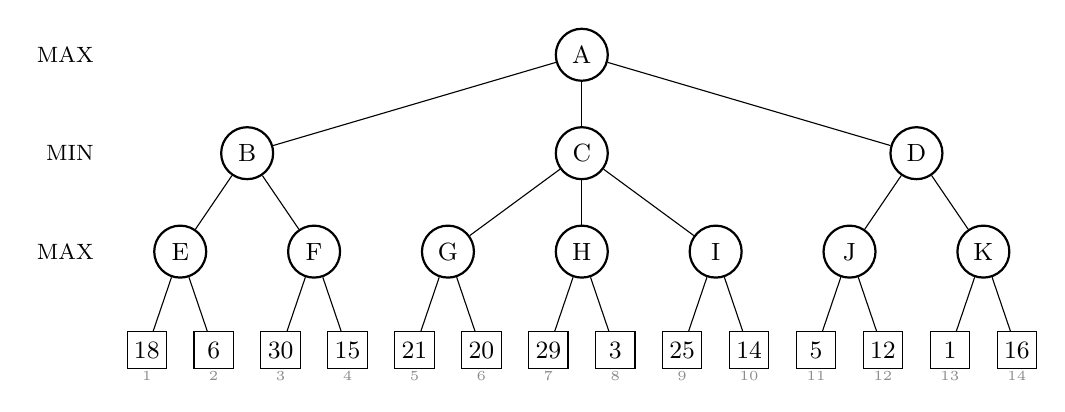
\begin{tikzpicture}[scale=1.0, every node/.style={transform shape}, gc/.style={draw, thick, circle, minimum size=6.6mm, inner sep=0pt, font=\small}, gl/.style={draw, rectangle, minimum width=5mm, minimum height=4.6mm, inner sep=1pt, font=\small}, gx/.style={draw=black!25, text=black!35}, val/.style={font=\footnotesize\bfseries, text=red!80!black, inner sep=1pt}]
\node[font=\footnotesize, anchor=east] at (-0.55,0.00) {MAX};
\node[font=\footnotesize, anchor=east] at (-0.55,-1.25) {MIN};
\node[font=\footnotesize, anchor=east] at (-0.55,-2.50) {MAX};
\node[gc] (n24) at (5.525,0.000) {A};
\node[gc] (n6) at (1.275,-1.250) {B};
\node[gc] (n2) at (0.425,-2.500) {E};
\node[gl, label={[font=\tiny, text=black!45, inner sep=1pt]below:1}] (n0) at (0.000,-3.750) {18};
\node[gl, label={[font=\tiny, text=black!45, inner sep=1pt]below:2}] (n1) at (0.850,-3.750) {6};
\node[gc] (n5) at (2.125,-2.500) {F};
\node[gl, label={[font=\tiny, text=black!45, inner sep=1pt]below:3}] (n3) at (1.700,-3.750) {30};
\node[gl, label={[font=\tiny, text=black!45, inner sep=1pt]below:4}] (n4) at (2.550,-3.750) {15};
\node[gc] (n16) at (5.525,-1.250) {C};
\node[gc] (n9) at (3.825,-2.500) {G};
\node[gl, label={[font=\tiny, text=black!45, inner sep=1pt]below:5}] (n7) at (3.400,-3.750) {21};
\node[gl, label={[font=\tiny, text=black!45, inner sep=1pt]below:6}] (n8) at (4.250,-3.750) {20};
\node[gc] (n12) at (5.525,-2.500) {H};
\node[gl, label={[font=\tiny, text=black!45, inner sep=1pt]below:7}] (n10) at (5.100,-3.750) {29};
\node[gl, label={[font=\tiny, text=black!45, inner sep=1pt]below:8}] (n11) at (5.950,-3.750) {3};
\node[gc] (n15) at (7.225,-2.500) {I};
\node[gl, label={[font=\tiny, text=black!45, inner sep=1pt]below:9}] (n13) at (6.800,-3.750) {25};
\node[gl, label={[font=\tiny, text=black!45, inner sep=1pt]below:10}] (n14) at (7.650,-3.750) {14};
\node[gc] (n23) at (9.775,-1.250) {D};
\node[gc] (n19) at (8.925,-2.500) {J};
\node[gl, label={[font=\tiny, text=black!45, inner sep=1pt]below:11}] (n17) at (8.500,-3.750) {5};
\node[gl, label={[font=\tiny, text=black!45, inner sep=1pt]below:12}] (n18) at (9.350,-3.750) {12};
\node[gc] (n22) at (10.625,-2.500) {K};
\node[gl, label={[font=\tiny, text=black!45, inner sep=1pt]below:13}] (n20) at (10.200,-3.750) {1};
\node[gl, label={[font=\tiny, text=black!45, inner sep=1pt]below:14}] (n21) at (11.050,-3.750) {16};
\draw (n24) -- (n6);
\draw (n24) -- (n16);
\draw (n24) -- (n23);
\draw (n6) -- (n2);
\draw (n6) -- (n5);
\draw (n2) -- (n0);
\draw (n2) -- (n1);
\draw (n5) -- (n3);
\draw (n5) -- (n4);
\draw (n16) -- (n9);
\draw (n16) -- (n12);
\draw (n16) -- (n15);
\draw (n9) -- (n7);
\draw (n9) -- (n8);
\draw (n12) -- (n10);
\draw (n12) -- (n11);
\draw (n15) -- (n13);
\draw (n15) -- (n14);
\draw (n23) -- (n19);
\draw (n23) -- (n22);
\draw (n19) -- (n17);
\draw (n19) -- (n18);
\draw (n22) -- (n20);
\draw (n22) -- (n21);
\end{tikzpicture}
\end{adjustbox}
\end{center}
\subq{(a)}Compute the final backed-up value of every node using the minimax algorithm (no alpha-beta pruning at this step). Which move should MAX make at the root?
\begin{solbox}
\begin{center}\small \begin{tabular}{|l|c|c|c|c|c|c|c|c|c|c|c|}\hline
\textbf{Node} & \textbf{A} & \textbf{B} & \textbf{C} & \textbf{D} & \textbf{E} & \textbf{F} & \textbf{G} & \textbf{H} & \textbf{I} & \textbf{J} & \textbf{K}\\ \hline
Minimax & \textcolor{blue!60!black}{21} & \textcolor{blue!60!black}{18} & \textcolor{blue!60!black}{21} & \textcolor{blue!60!black}{12} & \textcolor{blue!60!black}{18} & \textcolor{blue!60!black}{30} & \textcolor{blue!60!black}{21} & \textcolor{blue!60!black}{29} & \textcolor{blue!60!black}{25} & \textcolor{blue!60!black}{12} & \textcolor{blue!60!black}{16}\\[1.5mm] \hline
\end{tabular}\end{center}\begin{center}
\begin{adjustbox}{max width=\linewidth}
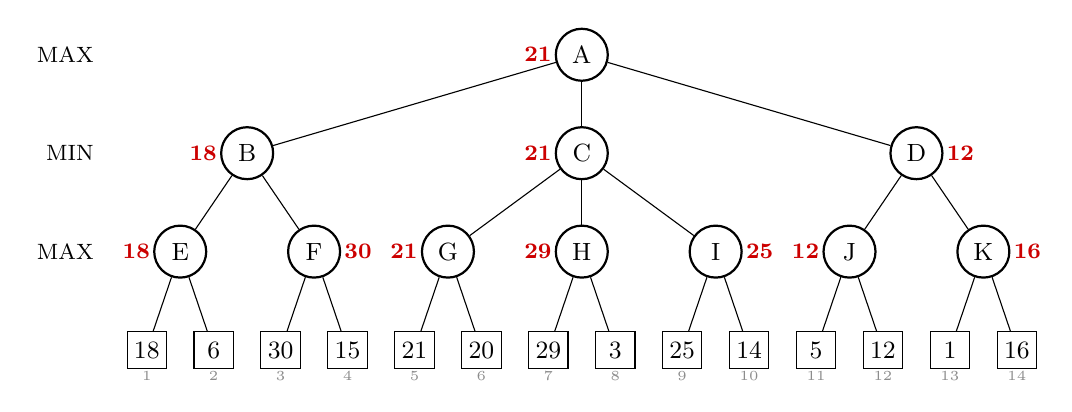
\begin{tikzpicture}[scale=1.0, every node/.style={transform shape}, gc/.style={draw, thick, circle, minimum size=6.6mm, inner sep=0pt, font=\small}, gl/.style={draw, rectangle, minimum width=5mm, minimum height=4.6mm, inner sep=1pt, font=\small}, gx/.style={draw=black!25, text=black!35}, val/.style={font=\footnotesize\bfseries, text=red!80!black, inner sep=1pt}]
\node[font=\footnotesize, anchor=east] at (-0.55,0.00) {MAX};
\node[font=\footnotesize, anchor=east] at (-0.55,-1.25) {MIN};
\node[font=\footnotesize, anchor=east] at (-0.55,-2.50) {MAX};
\node[gc, label={[val]left:21}] (n24) at (5.525,0.000) {A};
\node[gc, label={[val]left:18}] (n6) at (1.275,-1.250) {B};
\node[gc, label={[val]left:18}] (n2) at (0.425,-2.500) {E};
\node[gl, label={[font=\tiny, text=black!45, inner sep=1pt]below:1}] (n0) at (0.000,-3.750) {18};
\node[gl, label={[font=\tiny, text=black!45, inner sep=1pt]below:2}] (n1) at (0.850,-3.750) {6};
\node[gc, label={[val]right:30}] (n5) at (2.125,-2.500) {F};
\node[gl, label={[font=\tiny, text=black!45, inner sep=1pt]below:3}] (n3) at (1.700,-3.750) {30};
\node[gl, label={[font=\tiny, text=black!45, inner sep=1pt]below:4}] (n4) at (2.550,-3.750) {15};
\node[gc, label={[val]left:21}] (n16) at (5.525,-1.250) {C};
\node[gc, label={[val]left:21}] (n9) at (3.825,-2.500) {G};
\node[gl, label={[font=\tiny, text=black!45, inner sep=1pt]below:5}] (n7) at (3.400,-3.750) {21};
\node[gl, label={[font=\tiny, text=black!45, inner sep=1pt]below:6}] (n8) at (4.250,-3.750) {20};
\node[gc, label={[val]left:29}] (n12) at (5.525,-2.500) {H};
\node[gl, label={[font=\tiny, text=black!45, inner sep=1pt]below:7}] (n10) at (5.100,-3.750) {29};
\node[gl, label={[font=\tiny, text=black!45, inner sep=1pt]below:8}] (n11) at (5.950,-3.750) {3};
\node[gc, label={[val]right:25}] (n15) at (7.225,-2.500) {I};
\node[gl, label={[font=\tiny, text=black!45, inner sep=1pt]below:9}] (n13) at (6.800,-3.750) {25};
\node[gl, label={[font=\tiny, text=black!45, inner sep=1pt]below:10}] (n14) at (7.650,-3.750) {14};
\node[gc, label={[val]right:12}] (n23) at (9.775,-1.250) {D};
\node[gc, label={[val]left:12}] (n19) at (8.925,-2.500) {J};
\node[gl, label={[font=\tiny, text=black!45, inner sep=1pt]below:11}] (n17) at (8.500,-3.750) {5};
\node[gl, label={[font=\tiny, text=black!45, inner sep=1pt]below:12}] (n18) at (9.350,-3.750) {12};
\node[gc, label={[val]right:16}] (n22) at (10.625,-2.500) {K};
\node[gl, label={[font=\tiny, text=black!45, inner sep=1pt]below:13}] (n20) at (10.200,-3.750) {1};
\node[gl, label={[font=\tiny, text=black!45, inner sep=1pt]below:14}] (n21) at (11.050,-3.750) {16};
\draw (n24) -- (n6);
\draw (n24) -- (n16);
\draw (n24) -- (n23);
\draw (n6) -- (n2);
\draw (n6) -- (n5);
\draw (n2) -- (n0);
\draw (n2) -- (n1);
\draw (n5) -- (n3);
\draw (n5) -- (n4);
\draw (n16) -- (n9);
\draw (n16) -- (n12);
\draw (n16) -- (n15);
\draw (n9) -- (n7);
\draw (n9) -- (n8);
\draw (n12) -- (n10);
\draw (n12) -- (n11);
\draw (n15) -- (n13);
\draw (n15) -- (n14);
\draw (n23) -- (n19);
\draw (n23) -- (n22);
\draw (n19) -- (n17);
\draw (n19) -- (n18);
\draw (n22) -- (n20);
\draw (n22) -- (n21);
\end{tikzpicture}
\end{adjustbox}
\end{center}Root value $=21$; MAX moves to \textbf{C}.
\end{solbox}
\subq{(b)}Run alpha-beta pruning (children visited left to right). Give the value computed at every node (mark \textbf{X} if the node is never visited), cross out the pruned branches on the tree and briefly explain each case.
\begin{solbox}
\begin{center}\small \begin{tabular}{|l|c|c|c|c|c|c|c|c|c|c|c|}\hline
\textbf{Node} & \textbf{A} & \textbf{B} & \textbf{C} & \textbf{D} & \textbf{E} & \textbf{F} & \textbf{G} & \textbf{H} & \textbf{I} & \textbf{J} & \textbf{K}\\ \hline
$\alpha$-$\beta$ & \textcolor{blue!60!black}{$21$} & \textcolor{blue!60!black}{$18$} & \textcolor{blue!60!black}{$21$} & \textcolor{blue!60!black}{$\le 12$} & \textcolor{blue!60!black}{$18$} & \textcolor{blue!60!black}{$\ge 30$} & \textcolor{blue!60!black}{$21$} & \textcolor{blue!60!black}{$\ge 29$} & \textcolor{blue!60!black}{$\ge 25$} & \textcolor{blue!60!black}{$12$} & \textcolor{red!70!black}{\textbf{X}}\\[1.5mm] \hline
\end{tabular}\end{center}($\le v$ / $\ge v$: the node was cut off, so only this bound is known; writing the returned number $v$ is also accepted.)\begin{center}
\begin{adjustbox}{max width=\linewidth}
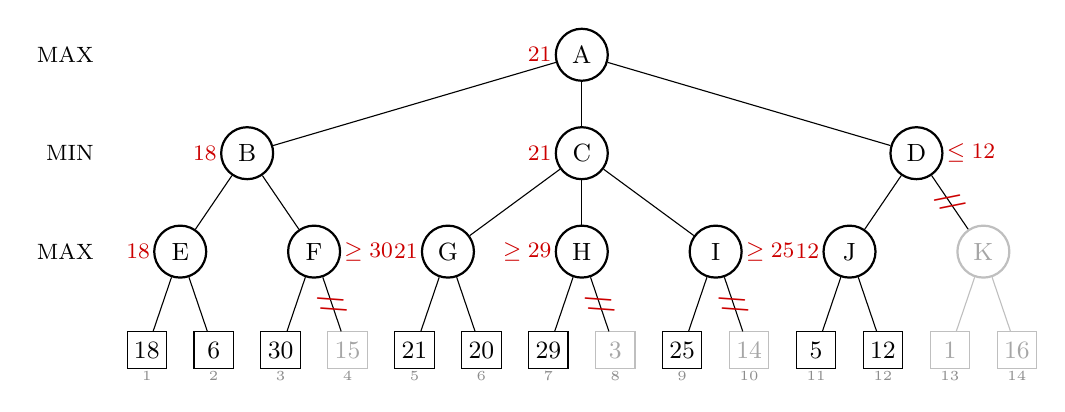
\begin{tikzpicture}[scale=1.0, every node/.style={transform shape}, gc/.style={draw, thick, circle, minimum size=6.6mm, inner sep=0pt, font=\small}, gl/.style={draw, rectangle, minimum width=5mm, minimum height=4.6mm, inner sep=1pt, font=\small}, gx/.style={draw=black!25, text=black!35}, val/.style={font=\footnotesize\bfseries, text=red!80!black, inner sep=1pt}]
\node[font=\footnotesize, anchor=east] at (-0.55,0.00) {MAX};
\node[font=\footnotesize, anchor=east] at (-0.55,-1.25) {MIN};
\node[font=\footnotesize, anchor=east] at (-0.55,-2.50) {MAX};
\node[gc, label={[val]left:$21$}] (n24) at (5.525,0.000) {A};
\node[gc, label={[val]left:$18$}] (n6) at (1.275,-1.250) {B};
\node[gc, label={[val]left:$18$}] (n2) at (0.425,-2.500) {E};
\node[gl, label={[font=\tiny, text=black!45, inner sep=1pt]below:1}] (n0) at (0.000,-3.750) {18};
\node[gl, label={[font=\tiny, text=black!45, inner sep=1pt]below:2}] (n1) at (0.850,-3.750) {6};
\node[gc, label={[val]right:$\ge30$}] (n5) at (2.125,-2.500) {F};
\node[gl, label={[font=\tiny, text=black!45, inner sep=1pt]below:3}] (n3) at (1.700,-3.750) {30};
\node[gl, gx, label={[font=\tiny, text=black!45, inner sep=1pt]below:4}] (n4) at (2.550,-3.750) {15};
\node[gc, label={[val]left:$21$}] (n16) at (5.525,-1.250) {C};
\node[gc, label={[val]left:$21$}] (n9) at (3.825,-2.500) {G};
\node[gl, label={[font=\tiny, text=black!45, inner sep=1pt]below:5}] (n7) at (3.400,-3.750) {21};
\node[gl, label={[font=\tiny, text=black!45, inner sep=1pt]below:6}] (n8) at (4.250,-3.750) {20};
\node[gc, label={[val]left:$\ge29$}] (n12) at (5.525,-2.500) {H};
\node[gl, label={[font=\tiny, text=black!45, inner sep=1pt]below:7}] (n10) at (5.100,-3.750) {29};
\node[gl, gx, label={[font=\tiny, text=black!45, inner sep=1pt]below:8}] (n11) at (5.950,-3.750) {3};
\node[gc, label={[val]right:$\ge25$}] (n15) at (7.225,-2.500) {I};
\node[gl, label={[font=\tiny, text=black!45, inner sep=1pt]below:9}] (n13) at (6.800,-3.750) {25};
\node[gl, gx, label={[font=\tiny, text=black!45, inner sep=1pt]below:10}] (n14) at (7.650,-3.750) {14};
\node[gc, label={[val]right:$\le12$}] (n23) at (9.775,-1.250) {D};
\node[gc, label={[val]left:$12$}] (n19) at (8.925,-2.500) {J};
\node[gl, label={[font=\tiny, text=black!45, inner sep=1pt]below:11}] (n17) at (8.500,-3.750) {5};
\node[gl, label={[font=\tiny, text=black!45, inner sep=1pt]below:12}] (n18) at (9.350,-3.750) {12};
\node[gc, gx] (n22) at (10.625,-2.500) {K};
\node[gl, gx, label={[font=\tiny, text=black!45, inner sep=1pt]below:13}] (n20) at (10.200,-3.750) {1};
\node[gl, gx, label={[font=\tiny, text=black!45, inner sep=1pt]below:14}] (n21) at (11.050,-3.750) {16};
\draw (n24) -- (n6);
\draw (n24) -- (n16);
\draw (n24) -- (n23);
\draw (n6) -- (n2);
\draw (n6) -- (n5);
\draw (n2) -- (n0);
\draw (n2) -- (n1);
\draw (n5) -- (n3);
\draw (n5) -- (n4) node[midway, sloped, text=red!80!black, font=\small\bfseries, inner sep=0pt]{/\!/};
\draw (n16) -- (n9);
\draw (n16) -- (n12);
\draw (n16) -- (n15);
\draw (n9) -- (n7);
\draw (n9) -- (n8);
\draw (n12) -- (n10);
\draw (n12) -- (n11) node[midway, sloped, text=red!80!black, font=\small\bfseries, inner sep=0pt]{/\!/};
\draw (n15) -- (n13);
\draw (n15) -- (n14) node[midway, sloped, text=red!80!black, font=\small\bfseries, inner sep=0pt]{/\!/};
\draw (n23) -- (n19);
\draw (n23) -- (n22) node[midway, sloped, text=red!80!black, font=\small\bfseries, inner sep=0pt]{/\!/};
\draw (n19) -- (n17);
\draw (n19) -- (n18);
\draw[black!25] (n22) -- (n20);
\draw[black!25] (n22) -- (n21);
\end{tikzpicture}
\end{adjustbox}
\end{center}$\alpha$ and $\beta$ at every visited node:\begin{center}\small\begin{tabular}{c c c c c}\toprule Node & Type & On entry & When it returns & Value returned\\\midrule A & MAX & $\alpha=-\infty,\ \beta=+\infty$ & $\alpha=21,\ \beta=+\infty$ & $21$ \\
B & MIN & $\alpha=-\infty,\ \beta=+\infty$ & $\alpha=-\infty,\ \beta=18$ & $18$ \\
E & MAX & $\alpha=-\infty,\ \beta=+\infty$ & $\alpha=18,\ \beta=+\infty$ & $18$ \\
F & MAX & $\alpha=-\infty,\ \beta=18$ & $\alpha=30,\ \beta=18$ & $\ge 30$ \\
C & MIN & $\alpha=18,\ \beta=+\infty$ & $\alpha=18,\ \beta=21$ & $21$ \\
G & MAX & $\alpha=18,\ \beta=+\infty$ & $\alpha=21,\ \beta=+\infty$ & $21$ \\
H & MAX & $\alpha=18,\ \beta=21$ & $\alpha=29,\ \beta=21$ & $\ge 29$ \\
I & MAX & $\alpha=18,\ \beta=21$ & $\alpha=25,\ \beta=21$ & $\ge 25$ \\
D & MIN & $\alpha=21,\ \beta=+\infty$ & $\alpha=21,\ \beta=12$ & $\le 12$ \\
J & MAX & $\alpha=21,\ \beta=+\infty$ & $\alpha=21,\ \beta=+\infty$ & $12$ \\\bottomrule\end{tabular}\end{center}\begin{itemize}[leftmargin=1.5em,itemsep=1pt]
\item At MAX node \textbf{F}, after leaf \#3: $v=30 \ge \beta=18$ $\Rightarrow$ prune leaf \#4. (MIN at B already has an alternative worth $\beta=18$, so it will never let play reach F.)
\item At MAX node \textbf{H}, after leaf \#7: $v=29 \ge \beta=21$ $\Rightarrow$ prune leaf \#8. (MIN at C already has an alternative worth $\beta=21$, so it will never let play reach H.)
\item At MAX node \textbf{I}, after leaf \#9: $v=25 \ge \beta=21$ $\Rightarrow$ prune leaf \#10. (MIN at C already has an alternative worth $\beta=21$, so it will never let play reach I.)
\item At MIN node \textbf{D}, after child J: $v=12 \le \alpha=21$ $\Rightarrow$ prune K (leaves \#13--\#14). (MAX at A already has an alternative worth $\alpha=21$, so it will never let play reach D.)
\end{itemize}Leaves evaluated: 9 of 14.
\end{solbox}
\subq{(c)}Using the minimax values from (a), and without performing any alpha-beta calculation, rotate the children of each node at every level so that alpha-beta prunes as much as possible. Draw the new tree (keep the node letters).
\begin{solbox}
Best child first for the player to move (MAX: largest value first, MIN: smallest first):\begin{center}
\begin{adjustbox}{max width=\linewidth}
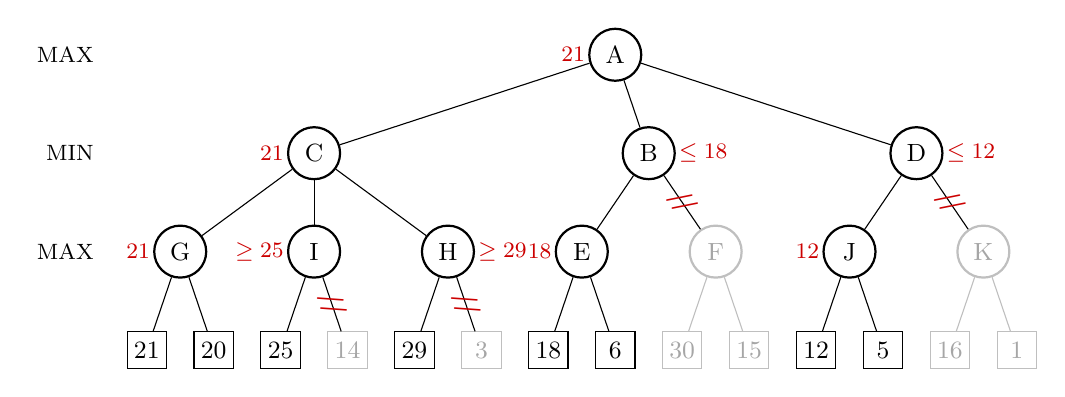
\begin{tikzpicture}[scale=1.0, every node/.style={transform shape}, gc/.style={draw, thick, circle, minimum size=6.6mm, inner sep=0pt, font=\small}, gl/.style={draw, rectangle, minimum width=5mm, minimum height=4.6mm, inner sep=1pt, font=\small}, gx/.style={draw=black!25, text=black!35}, val/.style={font=\footnotesize\bfseries, text=red!80!black, inner sep=1pt}]
\node[font=\footnotesize, anchor=east] at (-0.55,0.00) {MAX};
\node[font=\footnotesize, anchor=east] at (-0.55,-1.25) {MIN};
\node[font=\footnotesize, anchor=east] at (-0.55,-2.50) {MAX};
\node[gc, label={[val]left:$21$}] (n24) at (5.950,0.000) {A};
\node[gc, label={[val]left:$21$}] (n9) at (2.125,-1.250) {C};
\node[gc, label={[val]left:$21$}] (n2) at (0.425,-2.500) {G};
\node[gl] (n0) at (0.000,-3.750) {21};
\node[gl] (n1) at (0.850,-3.750) {20};
\node[gc, label={[val]left:$\ge25$}] (n5) at (2.125,-2.500) {I};
\node[gl] (n3) at (1.700,-3.750) {25};
\node[gl, gx] (n4) at (2.550,-3.750) {14};
\node[gc, label={[val]right:$\ge29$}] (n8) at (3.825,-2.500) {H};
\node[gl] (n6) at (3.400,-3.750) {29};
\node[gl, gx] (n7) at (4.250,-3.750) {3};
\node[gc, label={[val]right:$\le18$}] (n16) at (6.375,-1.250) {B};
\node[gc, label={[val]left:$18$}] (n12) at (5.525,-2.500) {E};
\node[gl] (n10) at (5.100,-3.750) {18};
\node[gl] (n11) at (5.950,-3.750) {6};
\node[gc, gx] (n15) at (7.225,-2.500) {F};
\node[gl, gx] (n13) at (6.800,-3.750) {30};
\node[gl, gx] (n14) at (7.650,-3.750) {15};
\node[gc, label={[val]right:$\le12$}] (n23) at (9.775,-1.250) {D};
\node[gc, label={[val]left:$12$}] (n19) at (8.925,-2.500) {J};
\node[gl] (n17) at (8.500,-3.750) {12};
\node[gl] (n18) at (9.350,-3.750) {5};
\node[gc, gx] (n22) at (10.625,-2.500) {K};
\node[gl, gx] (n20) at (10.200,-3.750) {16};
\node[gl, gx] (n21) at (11.050,-3.750) {1};
\draw (n24) -- (n9);
\draw (n24) -- (n16);
\draw (n24) -- (n23);
\draw (n9) -- (n2);
\draw (n9) -- (n5);
\draw (n9) -- (n8);
\draw (n2) -- (n0);
\draw (n2) -- (n1);
\draw (n5) -- (n3);
\draw (n5) -- (n4) node[midway, sloped, text=red!80!black, font=\small\bfseries, inner sep=0pt]{/\!/};
\draw (n8) -- (n6);
\draw (n8) -- (n7) node[midway, sloped, text=red!80!black, font=\small\bfseries, inner sep=0pt]{/\!/};
\draw (n16) -- (n12);
\draw (n16) -- (n15) node[midway, sloped, text=red!80!black, font=\small\bfseries, inner sep=0pt]{/\!/};
\draw (n12) -- (n10);
\draw (n12) -- (n11);
\draw[black!25] (n15) -- (n13);
\draw[black!25] (n15) -- (n14);
\draw (n23) -- (n19);
\draw (n23) -- (n22) node[midway, sloped, text=red!80!black, font=\small\bfseries, inner sep=0pt]{/\!/};
\draw (n19) -- (n17);
\draw (n19) -- (n18);
\draw[black!25] (n22) -- (n20);
\draw[black!25] (n22) -- (n21);
\end{tikzpicture}
\end{adjustbox}
\end{center}With this ordering alpha-beta evaluates only \textbf{8} leaves (instead of 9).
\end{solbox}
\question{5}Consider the game tree below, in which \textbf{MIN moves first} (the root is a MIN node).\begin{center}
\begin{adjustbox}{max width=\linewidth}
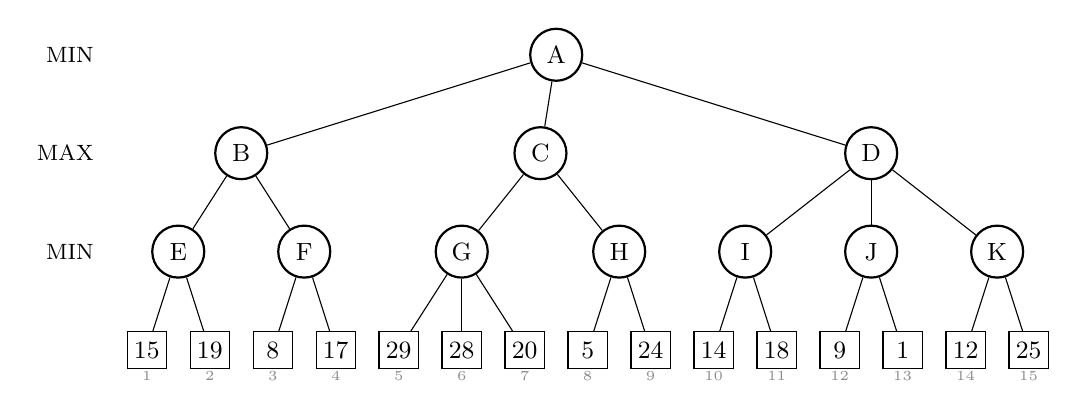
\begin{tikzpicture}[scale=1.0, every node/.style={transform shape}, gc/.style={draw, thick, circle, minimum size=6.6mm, inner sep=0pt, font=\small}, gl/.style={draw, rectangle, minimum width=5mm, minimum height=4.6mm, inner sep=1pt, font=\small}, gx/.style={draw=black!25, text=black!35}, val/.style={font=\footnotesize\bfseries, text=red!80!black, inner sep=1pt}]
\node[font=\footnotesize, anchor=east] at (-0.55,0.00) {MIN};
\node[font=\footnotesize, anchor=east] at (-0.55,-1.25) {MAX};
\node[font=\footnotesize, anchor=east] at (-0.55,-2.50) {MIN};
\node[gc] (n25) at (5.200,0.000) {A};
\node[gc] (n6) at (1.200,-1.250) {B};
\node[gc] (n2) at (0.400,-2.500) {E};
\node[gl, label={[font=\tiny, text=black!45, inner sep=1pt]below:1}] (n0) at (0.000,-3.750) {15};
\node[gl, label={[font=\tiny, text=black!45, inner sep=1pt]below:2}] (n1) at (0.800,-3.750) {19};
\node[gc] (n5) at (2.000,-2.500) {F};
\node[gl, label={[font=\tiny, text=black!45, inner sep=1pt]below:3}] (n3) at (1.600,-3.750) {8};
\node[gl, label={[font=\tiny, text=black!45, inner sep=1pt]below:4}] (n4) at (2.400,-3.750) {17};
\node[gc] (n14) at (5.000,-1.250) {C};
\node[gc] (n10) at (4.000,-2.500) {G};
\node[gl, label={[font=\tiny, text=black!45, inner sep=1pt]below:5}] (n7) at (3.200,-3.750) {29};
\node[gl, label={[font=\tiny, text=black!45, inner sep=1pt]below:6}] (n8) at (4.000,-3.750) {28};
\node[gl, label={[font=\tiny, text=black!45, inner sep=1pt]below:7}] (n9) at (4.800,-3.750) {20};
\node[gc] (n13) at (6.000,-2.500) {H};
\node[gl, label={[font=\tiny, text=black!45, inner sep=1pt]below:8}] (n11) at (5.600,-3.750) {5};
\node[gl, label={[font=\tiny, text=black!45, inner sep=1pt]below:9}] (n12) at (6.400,-3.750) {24};
\node[gc] (n24) at (9.200,-1.250) {D};
\node[gc] (n17) at (7.600,-2.500) {I};
\node[gl, label={[font=\tiny, text=black!45, inner sep=1pt]below:10}] (n15) at (7.200,-3.750) {14};
\node[gl, label={[font=\tiny, text=black!45, inner sep=1pt]below:11}] (n16) at (8.000,-3.750) {18};
\node[gc] (n20) at (9.200,-2.500) {J};
\node[gl, label={[font=\tiny, text=black!45, inner sep=1pt]below:12}] (n18) at (8.800,-3.750) {9};
\node[gl, label={[font=\tiny, text=black!45, inner sep=1pt]below:13}] (n19) at (9.600,-3.750) {1};
\node[gc] (n23) at (10.800,-2.500) {K};
\node[gl, label={[font=\tiny, text=black!45, inner sep=1pt]below:14}] (n21) at (10.400,-3.750) {12};
\node[gl, label={[font=\tiny, text=black!45, inner sep=1pt]below:15}] (n22) at (11.200,-3.750) {25};
\draw (n25) -- (n6);
\draw (n25) -- (n14);
\draw (n25) -- (n24);
\draw (n6) -- (n2);
\draw (n6) -- (n5);
\draw (n2) -- (n0);
\draw (n2) -- (n1);
\draw (n5) -- (n3);
\draw (n5) -- (n4);
\draw (n14) -- (n10);
\draw (n14) -- (n13);
\draw (n10) -- (n7);
\draw (n10) -- (n8);
\draw (n10) -- (n9);
\draw (n13) -- (n11);
\draw (n13) -- (n12);
\draw (n24) -- (n17);
\draw (n24) -- (n20);
\draw (n24) -- (n23);
\draw (n17) -- (n15);
\draw (n17) -- (n16);
\draw (n20) -- (n18);
\draw (n20) -- (n19);
\draw (n23) -- (n21);
\draw (n23) -- (n22);
\end{tikzpicture}
\end{adjustbox}
\end{center}
\subq{(a)}Note the minimax value of every node (no pruning).
\begin{solbox}
\begin{center}\small \begin{tabular}{|l|c|c|c|c|c|c|c|c|c|c|c|}\hline
\textbf{Node} & \textbf{A} & \textbf{B} & \textbf{C} & \textbf{D} & \textbf{E} & \textbf{F} & \textbf{G} & \textbf{H} & \textbf{I} & \textbf{J} & \textbf{K}\\ \hline
Minimax & \textcolor{blue!60!black}{14} & \textcolor{blue!60!black}{15} & \textcolor{blue!60!black}{20} & \textcolor{blue!60!black}{14} & \textcolor{blue!60!black}{15} & \textcolor{blue!60!black}{8} & \textcolor{blue!60!black}{20} & \textcolor{blue!60!black}{5} & \textcolor{blue!60!black}{14} & \textcolor{blue!60!black}{1} & \textcolor{blue!60!black}{12}\\[1.5mm] \hline
\end{tabular}\end{center}Root value $=14$; MIN moves to \textbf{D}.
\end{solbox}
\subq{(b)}Show where alpha-beta pruning occurs (left to right) by crossing out the corresponding branches, and briefly explain each case.
\begin{solbox}
\begin{center}
\begin{adjustbox}{max width=\linewidth}
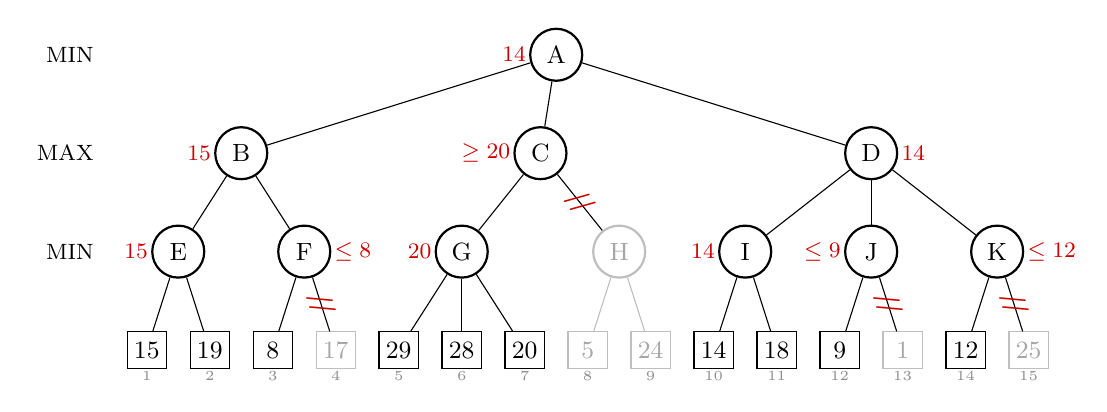
\begin{tikzpicture}[scale=1.0, every node/.style={transform shape}, gc/.style={draw, thick, circle, minimum size=6.6mm, inner sep=0pt, font=\small}, gl/.style={draw, rectangle, minimum width=5mm, minimum height=4.6mm, inner sep=1pt, font=\small}, gx/.style={draw=black!25, text=black!35}, val/.style={font=\footnotesize\bfseries, text=red!80!black, inner sep=1pt}]
\node[font=\footnotesize, anchor=east] at (-0.55,0.00) {MIN};
\node[font=\footnotesize, anchor=east] at (-0.55,-1.25) {MAX};
\node[font=\footnotesize, anchor=east] at (-0.55,-2.50) {MIN};
\node[gc, label={[val]left:$14$}] (n25) at (5.200,0.000) {A};
\node[gc, label={[val]left:$15$}] (n6) at (1.200,-1.250) {B};
\node[gc, label={[val]left:$15$}] (n2) at (0.400,-2.500) {E};
\node[gl, label={[font=\tiny, text=black!45, inner sep=1pt]below:1}] (n0) at (0.000,-3.750) {15};
\node[gl, label={[font=\tiny, text=black!45, inner sep=1pt]below:2}] (n1) at (0.800,-3.750) {19};
\node[gc, label={[val]right:$\le8$}] (n5) at (2.000,-2.500) {F};
\node[gl, label={[font=\tiny, text=black!45, inner sep=1pt]below:3}] (n3) at (1.600,-3.750) {8};
\node[gl, gx, label={[font=\tiny, text=black!45, inner sep=1pt]below:4}] (n4) at (2.400,-3.750) {17};
\node[gc, label={[val]left:$\ge20$}] (n14) at (5.000,-1.250) {C};
\node[gc, label={[val]left:$20$}] (n10) at (4.000,-2.500) {G};
\node[gl, label={[font=\tiny, text=black!45, inner sep=1pt]below:5}] (n7) at (3.200,-3.750) {29};
\node[gl, label={[font=\tiny, text=black!45, inner sep=1pt]below:6}] (n8) at (4.000,-3.750) {28};
\node[gl, label={[font=\tiny, text=black!45, inner sep=1pt]below:7}] (n9) at (4.800,-3.750) {20};
\node[gc, gx] (n13) at (6.000,-2.500) {H};
\node[gl, gx, label={[font=\tiny, text=black!45, inner sep=1pt]below:8}] (n11) at (5.600,-3.750) {5};
\node[gl, gx, label={[font=\tiny, text=black!45, inner sep=1pt]below:9}] (n12) at (6.400,-3.750) {24};
\node[gc, label={[val]right:$14$}] (n24) at (9.200,-1.250) {D};
\node[gc, label={[val]left:$14$}] (n17) at (7.600,-2.500) {I};
\node[gl, label={[font=\tiny, text=black!45, inner sep=1pt]below:10}] (n15) at (7.200,-3.750) {14};
\node[gl, label={[font=\tiny, text=black!45, inner sep=1pt]below:11}] (n16) at (8.000,-3.750) {18};
\node[gc, label={[val]left:$\le9$}] (n20) at (9.200,-2.500) {J};
\node[gl, label={[font=\tiny, text=black!45, inner sep=1pt]below:12}] (n18) at (8.800,-3.750) {9};
\node[gl, gx, label={[font=\tiny, text=black!45, inner sep=1pt]below:13}] (n19) at (9.600,-3.750) {1};
\node[gc, label={[val]right:$\le12$}] (n23) at (10.800,-2.500) {K};
\node[gl, label={[font=\tiny, text=black!45, inner sep=1pt]below:14}] (n21) at (10.400,-3.750) {12};
\node[gl, gx, label={[font=\tiny, text=black!45, inner sep=1pt]below:15}] (n22) at (11.200,-3.750) {25};
\draw (n25) -- (n6);
\draw (n25) -- (n14);
\draw (n25) -- (n24);
\draw (n6) -- (n2);
\draw (n6) -- (n5);
\draw (n2) -- (n0);
\draw (n2) -- (n1);
\draw (n5) -- (n3);
\draw (n5) -- (n4) node[midway, sloped, text=red!80!black, font=\small\bfseries, inner sep=0pt]{/\!/};
\draw (n14) -- (n10);
\draw (n14) -- (n13) node[midway, sloped, text=red!80!black, font=\small\bfseries, inner sep=0pt]{/\!/};
\draw (n10) -- (n7);
\draw (n10) -- (n8);
\draw (n10) -- (n9);
\draw[black!25] (n13) -- (n11);
\draw[black!25] (n13) -- (n12);
\draw (n24) -- (n17);
\draw (n24) -- (n20);
\draw (n24) -- (n23);
\draw (n17) -- (n15);
\draw (n17) -- (n16);
\draw (n20) -- (n18);
\draw (n20) -- (n19) node[midway, sloped, text=red!80!black, font=\small\bfseries, inner sep=0pt]{/\!/};
\draw (n23) -- (n21);
\draw (n23) -- (n22) node[midway, sloped, text=red!80!black, font=\small\bfseries, inner sep=0pt]{/\!/};
\end{tikzpicture}
\end{adjustbox}
\end{center}\begin{center}\small\begin{tabular}{c c c c c}\toprule Node & Type & On entry & When it returns & Value returned\\\midrule A & MIN & $\alpha=-\infty,\ \beta=+\infty$ & $\alpha=-\infty,\ \beta=14$ & $14$ \\
B & MAX & $\alpha=-\infty,\ \beta=+\infty$ & $\alpha=15,\ \beta=+\infty$ & $15$ \\
E & MIN & $\alpha=-\infty,\ \beta=+\infty$ & $\alpha=-\infty,\ \beta=15$ & $15$ \\
F & MIN & $\alpha=15,\ \beta=+\infty$ & $\alpha=15,\ \beta=8$ & $\le 8$ \\
C & MAX & $\alpha=-\infty,\ \beta=15$ & $\alpha=20,\ \beta=15$ & $\ge 20$ \\
G & MIN & $\alpha=-\infty,\ \beta=15$ & $\alpha=-\infty,\ \beta=15$ & $20$ \\
D & MAX & $\alpha=-\infty,\ \beta=15$ & $\alpha=14,\ \beta=15$ & $14$ \\
I & MIN & $\alpha=-\infty,\ \beta=15$ & $\alpha=-\infty,\ \beta=14$ & $14$ \\
J & MIN & $\alpha=14,\ \beta=15$ & $\alpha=14,\ \beta=9$ & $\le 9$ \\
K & MIN & $\alpha=14,\ \beta=15$ & $\alpha=14,\ \beta=12$ & $\le 12$ \\\bottomrule\end{tabular}\end{center}\begin{itemize}[leftmargin=1.5em,itemsep=1pt]
\item At MIN node \textbf{F}, after leaf \#3: $v=8 \le \alpha=15$ $\Rightarrow$ prune leaf \#4. (MAX at B already has an alternative worth $\alpha=15$, so it will never let play reach F.)
\item At MAX node \textbf{C}, after child G: $v=20 \ge \beta=15$ $\Rightarrow$ prune H (leaves \#8--\#9). (MIN at A already has an alternative worth $\beta=15$, so it will never let play reach C.)
\item At MIN node \textbf{J}, after leaf \#12: $v=9 \le \alpha=14$ $\Rightarrow$ prune leaf \#13. (MAX at D already has an alternative worth $\alpha=14$, so it will never let play reach J.)
\item At MIN node \textbf{K}, after leaf \#14: $v=12 \le \alpha=14$ $\Rightarrow$ prune leaf \#15. (MAX at D already has an alternative worth $\alpha=14$, so it will never let play reach K.)
\end{itemize}Leaves evaluated: 10 of 15; never evaluated: \#4, \#8, \#9, \#13, \#15.
\end{solbox}
\question{6}Consider the following game tree with chance nodes (outcome probabilities on the edges).\begin{center}
\begin{adjustbox}{max width=\linewidth}
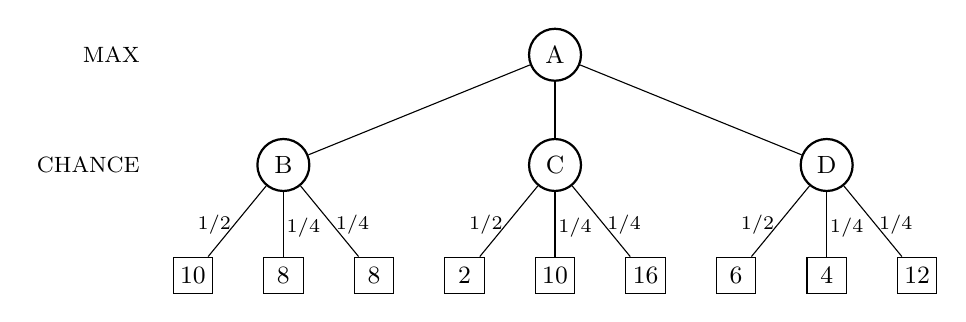
\begin{tikzpicture}[scale=1.0, every node/.style={transform shape}, gc/.style={draw, thick, circle, minimum size=6.6mm, inner sep=0pt, font=\small}, gl/.style={draw, rectangle, minimum width=5mm, minimum height=4.6mm, inner sep=1pt, font=\small}, gx/.style={draw=black!25, text=black!35}, val/.style={font=\footnotesize\bfseries, text=red!80!black, inner sep=1pt}]
\node[font=\footnotesize, anchor=east] at (-0.55,0.00) {MAX};
\node[font=\footnotesize, anchor=east] at (-0.55,-1.40) {CHANCE};
\node[gc] (n12) at (4.600,0.000) {A};
\node[gc] (n3) at (1.150,-1.400) {B};
\node[gl] (n0) at (0.000,-2.800) {10};
\node[gl] (n1) at (1.150,-2.800) {8};
\node[gl] (n2) at (2.300,-2.800) {8};
\node[gc] (n7) at (4.600,-1.400) {C};
\node[gl] (n4) at (3.450,-2.800) {2};
\node[gl] (n5) at (4.600,-2.800) {10};
\node[gl] (n6) at (5.750,-2.800) {16};
\node[gc] (n11) at (8.050,-1.400) {D};
\node[gl] (n8) at (6.900,-2.800) {6};
\node[gl] (n9) at (8.050,-2.800) {4};
\node[gl] (n10) at (9.200,-2.800) {12};
\draw (n12) -- (n3);
\draw (n12) -- (n7);
\draw (n12) -- (n11);
\draw (n3) -- (n0) node[pos=0.55, left, font=\scriptsize, inner sep=1pt]{$1/2$};
\draw (n3) -- (n1) node[pos=0.55, right, font=\scriptsize, inner sep=1pt]{$1/4$};
\draw (n3) -- (n2) node[pos=0.55, right, font=\scriptsize, inner sep=1pt]{$1/4$};
\draw (n7) -- (n4) node[pos=0.55, left, font=\scriptsize, inner sep=1pt]{$1/2$};
\draw (n7) -- (n5) node[pos=0.55, right, font=\scriptsize, inner sep=1pt]{$1/4$};
\draw (n7) -- (n6) node[pos=0.55, right, font=\scriptsize, inner sep=1pt]{$1/4$};
\draw (n11) -- (n8) node[pos=0.55, left, font=\scriptsize, inner sep=1pt]{$1/2$};
\draw (n11) -- (n9) node[pos=0.55, right, font=\scriptsize, inner sep=1pt]{$1/4$};
\draw (n11) -- (n10) node[pos=0.55, right, font=\scriptsize, inner sep=1pt]{$1/4$};
\end{tikzpicture}
\end{adjustbox}
\end{center}
\subq{(a)}Calculate the expectimax value of every node. Which move does MAX choose?
\begin{solbox}
\begin{center}
\begin{adjustbox}{max width=\linewidth}
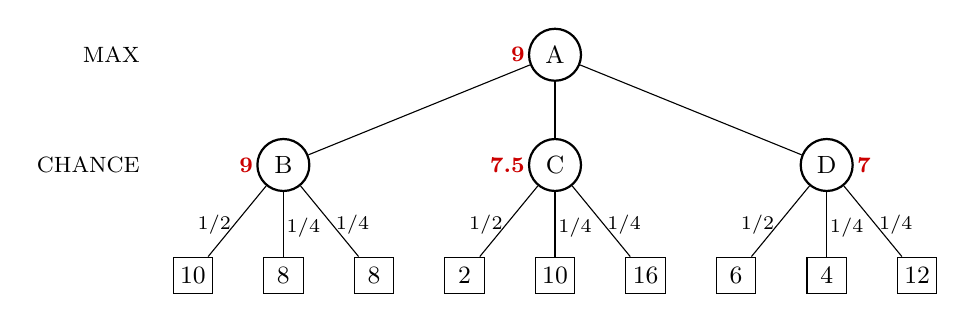
\begin{tikzpicture}[scale=1.0, every node/.style={transform shape}, gc/.style={draw, thick, circle, minimum size=6.6mm, inner sep=0pt, font=\small}, gl/.style={draw, rectangle, minimum width=5mm, minimum height=4.6mm, inner sep=1pt, font=\small}, gx/.style={draw=black!25, text=black!35}, val/.style={font=\footnotesize\bfseries, text=red!80!black, inner sep=1pt}]
\node[font=\footnotesize, anchor=east] at (-0.55,0.00) {MAX};
\node[font=\footnotesize, anchor=east] at (-0.55,-1.40) {CHANCE};
\node[gc, label={[val]left:9}] (n12) at (4.600,0.000) {A};
\node[gc, label={[val]left:9}] (n3) at (1.150,-1.400) {B};
\node[gl] (n0) at (0.000,-2.800) {10};
\node[gl] (n1) at (1.150,-2.800) {8};
\node[gl] (n2) at (2.300,-2.800) {8};
\node[gc, label={[val]left:7.5}] (n7) at (4.600,-1.400) {C};
\node[gl] (n4) at (3.450,-2.800) {2};
\node[gl] (n5) at (4.600,-2.800) {10};
\node[gl] (n6) at (5.750,-2.800) {16};
\node[gc, label={[val]right:7}] (n11) at (8.050,-1.400) {D};
\node[gl] (n8) at (6.900,-2.800) {6};
\node[gl] (n9) at (8.050,-2.800) {4};
\node[gl] (n10) at (9.200,-2.800) {12};
\draw (n12) -- (n3);
\draw (n12) -- (n7);
\draw (n12) -- (n11);
\draw (n3) -- (n0) node[pos=0.55, left, font=\scriptsize, inner sep=1pt]{$1/2$};
\draw (n3) -- (n1) node[pos=0.55, right, font=\scriptsize, inner sep=1pt]{$1/4$};
\draw (n3) -- (n2) node[pos=0.55, right, font=\scriptsize, inner sep=1pt]{$1/4$};
\draw (n7) -- (n4) node[pos=0.55, left, font=\scriptsize, inner sep=1pt]{$1/2$};
\draw (n7) -- (n5) node[pos=0.55, right, font=\scriptsize, inner sep=1pt]{$1/4$};
\draw (n7) -- (n6) node[pos=0.55, right, font=\scriptsize, inner sep=1pt]{$1/4$};
\draw (n11) -- (n8) node[pos=0.55, left, font=\scriptsize, inner sep=1pt]{$1/2$};
\draw (n11) -- (n9) node[pos=0.55, right, font=\scriptsize, inner sep=1pt]{$1/4$};
\draw (n11) -- (n10) node[pos=0.55, right, font=\scriptsize, inner sep=1pt]{$1/4$};
\end{tikzpicture}
\end{adjustbox}
\end{center}B $=1/2\cdot10+1/4\cdot8+1/4\cdot8=9$; C $=1/2\cdot2+1/4\cdot10+1/4\cdot16=7.5$; D $=1/2\cdot6+1/4\cdot4+1/4\cdot12=7$. MAX chooses \textbf{B} (9).
\end{solbox}
\subq{(b)}Which move would MAX choose if the chance nodes were MIN nodes?
\begin{solbox}
B$=8$, C$=2$, D$=4$ $\Rightarrow$ B.
\end{solbox}
\subq{(c)}Replace every leaf value $x$ by $x^2$ (order-preserving for these positive values). Does the expectimax decision change? What does this tell you about evaluation functions in stochastic games?
\begin{solbox}
B $=82$, C $=91$, D $=58$ $\Rightarrow$ MAX now chooses \textbf{C}: the decision changes. For expectimax the magnitudes of the values matter (only a positive linear transformation is safe), whereas minimax only needs the order.
\end{solbox}
\question{7}Consider the MCTS tree below; rollouts return 1 (win for the root player) or 0 (loss), $t$ is the total reward and $n$ the number of visits. Use $\mathrm{UCB1}=\bar V_i + C\sqrt{\ln N/n_i}$ with $C=\sqrt2$ (unvisited $=\infty$, ties to the left). A leaf never visited is rolled out directly; otherwise all its children are added and the rollout starts at the first. Expansions create: $A_1\to A_3,A_4$; $A_2\to A_5,A_6$; $B_1\to B_3,B_4$; $B_2\to B_5,B_6$; $C_1\to C_3,C_4$; $C_2\to C_5,C_6$.\begin{center}
\begin{adjustbox}{max width=\linewidth}
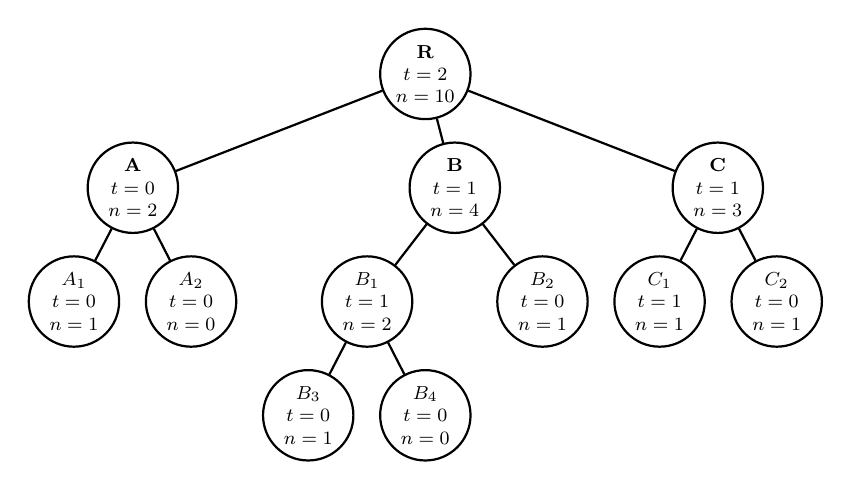
\begin{tikzpicture}[scale=0.85, every node/.style={transform shape}, mn/.style={draw, thick, circle, align=center, font=\footnotesize, inner sep=0.5pt, minimum size=13.5mm}]
\node[mn] (m1) at (5.25,0.00) {\textbf{R}\\ $t=2$\\ $n=10$};
\node[mn] (m2) at (0.88,-1.70) {\textbf{A}\\ $t=0$\\ $n=2$};
\node[mn] (m3) at (0.00,-3.40) {\textbf{$A_{1}$}\\ $t=0$\\ $n=1$};
\draw[thick] (m2) -- (m3);
\node[mn] (m4) at (1.75,-3.40) {\textbf{$A_{2}$}\\ $t=0$\\ $n=0$};
\draw[thick] (m2) -- (m4);
\draw[thick] (m1) -- (m2);
\node[mn] (m5) at (5.69,-1.70) {\textbf{B}\\ $t=1$\\ $n=4$};
\node[mn] (m6) at (4.38,-3.40) {\textbf{$B_{1}$}\\ $t=1$\\ $n=2$};
\node[mn] (m7) at (3.50,-5.10) {\textbf{$B_{3}$}\\ $t=0$\\ $n=1$};
\draw[thick] (m6) -- (m7);
\node[mn] (m8) at (5.25,-5.10) {\textbf{$B_{4}$}\\ $t=0$\\ $n=0$};
\draw[thick] (m6) -- (m8);
\draw[thick] (m5) -- (m6);
\node[mn] (m9) at (7.00,-3.40) {\textbf{$B_{2}$}\\ $t=0$\\ $n=1$};
\draw[thick] (m5) -- (m9);
\draw[thick] (m1) -- (m5);
\node[mn] (m10) at (9.62,-1.70) {\textbf{C}\\ $t=1$\\ $n=3$};
\node[mn] (m11) at (8.75,-3.40) {\textbf{$C_{1}$}\\ $t=1$\\ $n=1$};
\draw[thick] (m10) -- (m11);
\node[mn] (m12) at (10.50,-3.40) {\textbf{$C_{2}$}\\ $t=0$\\ $n=1$};
\draw[thick] (m10) -- (m12);
\draw[thick] (m1) -- (m10);
\end{tikzpicture}
\end{adjustbox}
\end{center}
\subq{(a)}Calculate UCB1 for $A$, $B$ and $C$. Which child is selected?
\begin{solbox}
A: $\frac{0}{2} + \sqrt2\sqrt{\frac{\ln 10}{2}} = 1.517$; B: $\frac{1}{4} + \sqrt2\sqrt{\frac{\ln 10}{4}} = 1.323$; C: $\frac{1}{3} + \sqrt2\sqrt{\frac{\ln 10}{3}} = 1.572$ $\Rightarrow$ \textbf{C}.
\end{solbox}
\subq{(b)}Perform three iterations whose rollouts return $1,\ 0,\ 0$ (in order); update the statistics and draw the final tree.
\begin{solbox}
\textbf{Iteration 1.}
\begin{itemize}[leftmargin=1.5em,itemsep=1pt]
\item \emph{Selection} at R ($N=10$): A: $\frac{0}{2} + \sqrt2\sqrt{\frac{\ln 10}{2}} = 1.517$; B: $\frac{1}{4} + \sqrt2\sqrt{\frac{\ln 10}{4}} = 1.323$; C: $\frac{1}{3} + \sqrt2\sqrt{\frac{\ln 10}{3}} = 1.572$ $\Rightarrow$ go to \textbf{C}.
\item \emph{Selection} at C ($N=3$): $C_{1}$: $\frac{1}{1} + \sqrt2\sqrt{\frac{\ln 3}{1}} = 2.482$; $C_{2}$: $\frac{0}{1} + \sqrt2\sqrt{\frac{\ln 3}{1}} = 1.482$ $\Rightarrow$ go to \textbf{$C_{1}$}.
\item \emph{Expansion}: $C_{1}$ was visited before ($n>0$) and has no children $\Rightarrow$ add $C_{3}$, $C_{4}$; roll out from the first one, \textbf{$C_{3}$}.
\item \emph{Simulation}: rollout from $C_{3}$ returns $1$.
\item \emph{Backpropagation}: add $1$ to $t$ and $1$ to $n$ for R $\to$ C $\to$ $C_{1}$ $\to$ $C_{3}$.
\end{itemize}
\textit{Statistics ($t/n$) after iteration 1:} R: 3/11, A: 0/2, $A_{1}$: 0/1, $A_{2}$: 0/0, B: 1/4, $B_{1}$: 1/2, $B_{3}$: 0/1, $B_{4}$: 0/0, $B_{2}$: 0/1, C: 2/4, $C_{1}$: 2/2, $C_{3}$: 1/1, $C_{4}$: 0/0, $C_{2}$: 0/1.

\smallskip
\textbf{Iteration 2.}
\begin{itemize}[leftmargin=1.5em,itemsep=1pt]
\item \emph{Selection} at R ($N=11$): A: $\frac{0}{2} + \sqrt2\sqrt{\frac{\ln 11}{2}} = 1.549$; B: $\frac{1}{4} + \sqrt2\sqrt{\frac{\ln 11}{4}} = 1.345$; C: $\frac{2}{4} + \sqrt2\sqrt{\frac{\ln 11}{4}} = 1.595$ $\Rightarrow$ go to \textbf{C}.
\item \emph{Selection} at C ($N=4$): $C_{1}$: $\frac{2}{2} + \sqrt2\sqrt{\frac{\ln 4}{2}} = 2.177$; $C_{2}$: $\frac{0}{1} + \sqrt2\sqrt{\frac{\ln 4}{1}} = 1.665$ $\Rightarrow$ go to \textbf{$C_{1}$}.
\item \emph{Selection} at $C_{1}$ ($N=2$): $C_{3}$: $\frac{1}{1} + \sqrt2\sqrt{\frac{\ln 2}{1}} = 2.177$; $C_{4}$: $\infty$ (unvisited) $\Rightarrow$ go to \textbf{$C_{4}$}.
\item \emph{Expansion}: none --- \textbf{$C_{4}$} has $n=0$, so we roll out directly from it.
\item \emph{Simulation}: rollout from $C_{4}$ returns $0$.
\item \emph{Backpropagation}: add $0$ to $t$ and $1$ to $n$ for R $\to$ C $\to$ $C_{1}$ $\to$ $C_{4}$.
\end{itemize}
\textit{Statistics ($t/n$) after iteration 2:} R: 3/12, A: 0/2, $A_{1}$: 0/1, $A_{2}$: 0/0, B: 1/4, $B_{1}$: 1/2, $B_{3}$: 0/1, $B_{4}$: 0/0, $B_{2}$: 0/1, C: 2/5, $C_{1}$: 2/3, $C_{3}$: 1/1, $C_{4}$: 0/1, $C_{2}$: 0/1.

\smallskip
\textbf{Iteration 3.}
\begin{itemize}[leftmargin=1.5em,itemsep=1pt]
\item \emph{Selection} at R ($N=12$): A: $\frac{0}{2} + \sqrt2\sqrt{\frac{\ln 12}{2}} = 1.576$; B: $\frac{1}{4} + \sqrt2\sqrt{\frac{\ln 12}{4}} = 1.365$; C: $\frac{2}{5} + \sqrt2\sqrt{\frac{\ln 12}{5}} = 1.397$ $\Rightarrow$ go to \textbf{A}.
\item \emph{Selection} at A ($N=2$): $A_{1}$: $\frac{0}{1} + \sqrt2\sqrt{\frac{\ln 2}{1}} = 1.177$; $A_{2}$: $\infty$ (unvisited) $\Rightarrow$ go to \textbf{$A_{2}$}.
\item \emph{Expansion}: none --- \textbf{$A_{2}$} has $n=0$, so we roll out directly from it.
\item \emph{Simulation}: rollout from $A_{2}$ returns $0$.
\item \emph{Backpropagation}: add $0$ to $t$ and $1$ to $n$ for R $\to$ A $\to$ $A_{2}$.
\end{itemize}
\textit{Statistics ($t/n$) after iteration 3:} R: 3/13, A: 0/3, $A_{1}$: 0/1, $A_{2}$: 0/1, B: 1/4, $B_{1}$: 1/2, $B_{3}$: 0/1, $B_{4}$: 0/0, $B_{2}$: 0/1, C: 2/5, $C_{1}$: 2/3, $C_{3}$: 1/1, $C_{4}$: 0/1, $C_{2}$: 0/1.\par Final tree:\begin{center}
\begin{adjustbox}{max width=\linewidth}
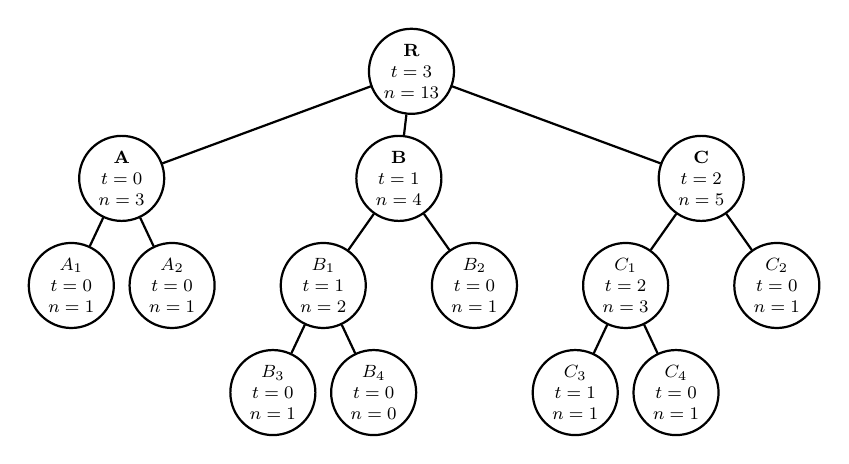
\begin{tikzpicture}[scale=0.8, every node/.style={transform shape}, mn/.style={draw, thick, circle, align=center, font=\footnotesize, inner sep=0.5pt, minimum size=13.5mm}]
\node[mn] (m1) at (5.40,0.00) {\textbf{R}\\ $t=3$\\ $n=13$};
\node[mn] (m2) at (0.80,-1.70) {\textbf{A}\\ $t=0$\\ $n=3$};
\node[mn] (m3) at (0.00,-3.40) {\textbf{$A_{1}$}\\ $t=0$\\ $n=1$};
\draw[thick] (m2) -- (m3);
\node[mn] (m4) at (1.60,-3.40) {\textbf{$A_{2}$}\\ $t=0$\\ $n=1$};
\draw[thick] (m2) -- (m4);
\draw[thick] (m1) -- (m2);
\node[mn] (m5) at (5.20,-1.70) {\textbf{B}\\ $t=1$\\ $n=4$};
\node[mn] (m6) at (4.00,-3.40) {\textbf{$B_{1}$}\\ $t=1$\\ $n=2$};
\node[mn] (m7) at (3.20,-5.10) {\textbf{$B_{3}$}\\ $t=0$\\ $n=1$};
\draw[thick] (m6) -- (m7);
\node[mn] (m8) at (4.80,-5.10) {\textbf{$B_{4}$}\\ $t=0$\\ $n=0$};
\draw[thick] (m6) -- (m8);
\draw[thick] (m5) -- (m6);
\node[mn] (m9) at (6.40,-3.40) {\textbf{$B_{2}$}\\ $t=0$\\ $n=1$};
\draw[thick] (m5) -- (m9);
\draw[thick] (m1) -- (m5);
\node[mn] (m10) at (10.00,-1.70) {\textbf{C}\\ $t=2$\\ $n=5$};
\node[mn] (m11) at (8.80,-3.40) {\textbf{$C_{1}$}\\ $t=2$\\ $n=3$};
\node[mn] (m12) at (8.00,-5.10) {\textbf{$C_{3}$}\\ $t=1$\\ $n=1$};
\draw[thick] (m11) -- (m12);
\node[mn] (m13) at (9.60,-5.10) {\textbf{$C_{4}$}\\ $t=0$\\ $n=1$};
\draw[thick] (m11) -- (m13);
\draw[thick] (m10) -- (m11);
\node[mn] (m14) at (11.20,-3.40) {\textbf{$C_{2}$}\\ $t=0$\\ $n=1$};
\draw[thick] (m10) -- (m14);
\draw[thick] (m1) -- (m10);
\end{tikzpicture}
\end{adjustbox}
\end{center}
\end{solbox}
\subq{(c)}If the search stopped now, which move is played by the robust-child rule (the lecture's \texttt{best\_child})? Does the max-child rule agree?
\begin{solbox}
A: $0/3$, B: $1/4$, C: $2/5$ $\Rightarrow$ robust child \textbf{C}; max child \textbf{C}.
\end{solbox}
\question{8}This problem is about map colouring. Each region must be coloured Red (R), Green (G) or Blue (B), and neighbouring regions must have different colours. The constraint graph is shown below. The following questions are mutually independent.\begin{center}
\begin{adjustbox}{max width=\linewidth}
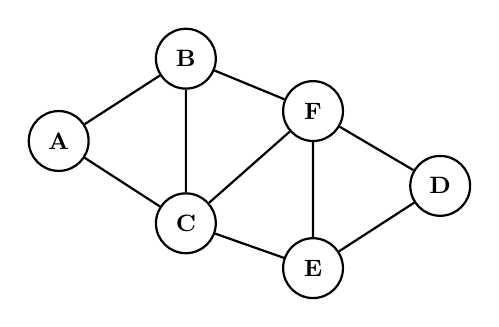
\begin{tikzpicture}[scale=0.95, every node/.style={transform shape}, cv/.style={draw, thick, circle, minimum size=8mm, inner sep=0pt, font=\small\bfseries}]
\node[cv] (A) at (0.00,1.00) {A};
\node[cv] (B) at (1.70,2.10) {B};
\node[cv] (C) at (1.70,-0.10) {C};
\node[cv] (F) at (3.40,1.40) {F};
\node[cv] (E) at (3.40,-0.70) {E};
\node[cv] (D) at (5.10,0.40) {D};
\draw[thick] (A) to[] (B);
\draw[thick] (A) to[] (C);
\draw[thick] (B) to[] (C);
\draw[thick] (B) to[] (F);
\draw[thick] (C) to[] (E);
\draw[thick] (C) to[] (F);
\draw[thick] (D) to[] (E);
\draw[thick] (D) to[] (F);
\draw[thick] (E) to[] (F);
\end{tikzpicture}
\end{adjustbox}
\end{center}
\subq{(a)}\textbf{Cross out} all values that would be eliminated by \emph{forward checking} after variable B has been assigned as shown.\begin{center}\small\begin{tabular}{|l|c|c|c|c|c|c|}\hline Variables & \textbf{A} & \textbf{B} & \textbf{C} & \textbf{D} & \textbf{E} & \textbf{F}\\ \hline Domains & R\ G\ B & \textbf{R} & R\ G\ B & R\ G\ B & R\ G\ B & R\ G\ B\\ \hline\end{tabular}\end{center}
\begin{solbox}
\begin{center}\small\begin{tabular}{|l|c|c|c|c|c|c|}\hline Variables & \textbf{A} & \textbf{B} & \textbf{C} & \textbf{D} & \textbf{E} & \textbf{F}\\ \hline Domains & \textcolor{red!70!black}{\sout{R}}\ G\ B & \textbf{R}\ \textcolor{red!70!black}{\sout{G}}\ \textcolor{red!70!black}{\sout{B}} & \textcolor{red!70!black}{\sout{R}}\ G\ B & R\ G\ B & R\ G\ B & \textcolor{red!70!black}{\sout{R}}\ G\ B\\ \hline\end{tabular}\end{center}Only the neighbours of B (A, C, F) lose R.
\end{solbox}
\subq{(b)}A and B have been assigned as shown, but no constraint propagation has been done yet. \textbf{Cross out} all values that would be eliminated by \emph{arc consistency} (AC-3).\begin{center}\small\begin{tabular}{|l|c|c|c|c|c|c|}\hline Variables & \textbf{A} & \textbf{B} & \textbf{C} & \textbf{D} & \textbf{E} & \textbf{F}\\ \hline Domains & \textbf{R} & \textbf{G} & R\ G\ B & R\ G\ B & R\ G\ B & R\ G\ B\\ \hline\end{tabular}\end{center}
\begin{solbox}
\begin{center}\small\begin{tabular}{|l|c|c|c|c|c|c|}\hline Variables & \textbf{A} & \textbf{B} & \textbf{C} & \textbf{D} & \textbf{E} & \textbf{F}\\ \hline Domains & \textbf{R}\ \textcolor{red!70!black}{\sout{G}}\ \textcolor{red!70!black}{\sout{B}} & \textcolor{red!70!black}{\sout{R}}\ \textbf{G}\ \textcolor{red!70!black}{\sout{B}} & \textcolor{red!70!black}{\sout{R}}\ \textcolor{red!70!black}{\sout{G}}\ B & \textcolor{red!70!black}{\sout{R}}\ \textcolor{red!70!black}{\sout{G}}\ B & \textcolor{red!70!black}{\sout{R}}\ G\ \textcolor{red!70!black}{\sout{B}} & R\ \textcolor{red!70!black}{\sout{G}}\ \textcolor{red!70!black}{\sout{B}}\\ \hline\end{tabular}\end{center}Propagation continues through the graph (unlike forward checking): every arc $X_i\to X_j$ is revised until no domain changes. Here arc consistency even leaves a single value for every variable.
\end{solbox}
\subq{(c)}Variable A is already assigned and constraint propagation has been done. \textbf{Circle} all unassigned variables that might be selected by the \emph{Minimum-Remaining-Values} (MRV) heuristic.\begin{center}\small\begin{tabular}{|l|c|c|c|c|c|c|}\hline Variables & \textbf{A} & \textbf{B} & \textbf{C} & \textbf{D} & \textbf{E} & \textbf{F}\\ \hline Domains & \textbf{R} & G\ B & G\ B & R\ G\ B & R\ G\ B & R\ G\ B\\ \hline\end{tabular}\end{center}
\begin{solbox}
Remaining values: B: 2, C: 2, D: 3, E: 3, F: 3 $\Rightarrow$ MRV may select \textbf{B, C}.
\end{solbox}
\subq{(d)}Same situation. \textbf{Circle} all unassigned variables that might be selected by the \emph{Degree Heuristic}.\begin{center}\small\begin{tabular}{|l|c|c|c|c|c|c|}\hline Variables & \textbf{A} & \textbf{B} & \textbf{C} & \textbf{D} & \textbf{E} & \textbf{F}\\ \hline Domains & \textbf{R} & G\ B & G\ B & R\ G\ B & R\ G\ B & R\ G\ B\\ \hline\end{tabular}\end{center}
\begin{solbox}
Degree = number of constraints with other \emph{unassigned} variables: B: 2, C: 3, D: 2, E: 3, F: 4 $\Rightarrow$ the degree heuristic may select \textbf{F}.
\end{solbox}
\subq{(e)}Assume no variable has been assigned yet. Solve the CSP using backtracking with \emph{forward checking}, choosing variables with MRV, then the degree heuristic (DH), and finally alphabetical order; try values in the order R, G, B. For every step give the MRV value of every region not yet coloured, and the DH values of the regions tied on the minimum MRV.
\begin{solbox}
\par \underline{Step 1}\par\begin{center}\small \begin{tabular}{|l|c|c|c|c|c|c|}\hline Variables & \textbf{A} & \textbf{B} & \textbf{C} & \textbf{D} & \textbf{E} & \textbf{F}\\ \hline MRV & \textcolor{blue!60!black}{3} & \textcolor{blue!60!black}{3} & \textcolor{blue!60!black}{3} & \textcolor{blue!60!black}{3} & \textcolor{blue!60!black}{3} & \textcolor{blue!60!black}{3}\\ \hline DH & \textcolor{blue!60!black}{2} & \textcolor{blue!60!black}{3} & \textcolor{blue!60!black}{4} & \textcolor{blue!60!black}{2} & \textcolor{blue!60!black}{3} & \textcolor{blue!60!black}{4}\\ \hline\end{tabular}\end{center}Assign to the variable \textbf{C} with the value \textbf{R} (tie on MRV and DH, broken alphabetically). Domains before this step: A=RGB, B=RGB, C=RGB, D=RGB, E=RGB, F=RGB.\par
\underline{Step 2}\par\begin{center}\small \begin{tabular}{|l|c|c|c|c|c|c|}\hline Variables & \textbf{A} & \textbf{B} & \textbf{C} & \textbf{D} & \textbf{E} & \textbf{F}\\ \hline MRV & \textcolor{blue!60!black}{2} & \textcolor{blue!60!black}{2} & -- & \textcolor{blue!60!black}{3} & \textcolor{blue!60!black}{2} & \textcolor{blue!60!black}{2}\\ \hline DH & \textcolor{blue!60!black}{1} & \textcolor{blue!60!black}{2} &  &  & \textcolor{blue!60!black}{2} & \textcolor{blue!60!black}{3}\\ \hline\end{tabular}\end{center}Assign to the variable \textbf{F} with the value \textbf{G} (tie on MRV broken by DH). Domains before this step: A=GB, B=GB, C=R, D=RGB, E=GB, F=GB.\par
\underline{Step 3}\par\begin{center}\small \begin{tabular}{|l|c|c|c|c|c|c|}\hline Variables & \textbf{A} & \textbf{B} & \textbf{C} & \textbf{D} & \textbf{E} & \textbf{F}\\ \hline MRV & \textcolor{blue!60!black}{2} & \textcolor{blue!60!black}{1} & -- & \textcolor{blue!60!black}{2} & \textcolor{blue!60!black}{1} & --\\ \hline DH &  & \textcolor{blue!60!black}{1} &  &  & \textcolor{blue!60!black}{1} & \\ \hline\end{tabular}\end{center}Assign to the variable \textbf{B} with the value \textbf{B} (tie on MRV and DH, broken alphabetically). Domains before this step: A=GB, B=B, C=R, D=RB, E=B, F=G.\par
\underline{Step 4}\par\begin{center}\small \begin{tabular}{|l|c|c|c|c|c|c|}\hline Variables & \textbf{A} & \textbf{B} & \textbf{C} & \textbf{D} & \textbf{E} & \textbf{F}\\ \hline MRV & \textcolor{blue!60!black}{1} & -- & -- & \textcolor{blue!60!black}{2} & \textcolor{blue!60!black}{1} & --\\ \hline DH & \textcolor{blue!60!black}{0} &  &  &  & \textcolor{blue!60!black}{1} & \\ \hline\end{tabular}\end{center}Assign to the variable \textbf{E} with the value \textbf{B} (tie on MRV broken by DH). Domains before this step: A=G, B=B, C=R, D=RB, E=B, F=G.\par
\underline{Step 5}\par\begin{center}\small \begin{tabular}{|l|c|c|c|c|c|c|}\hline Variables & \textbf{A} & \textbf{B} & \textbf{C} & \textbf{D} & \textbf{E} & \textbf{F}\\ \hline MRV & \textcolor{blue!60!black}{1} & -- & -- & \textcolor{blue!60!black}{1} & -- & --\\ \hline DH & \textcolor{blue!60!black}{0} &  &  & \textcolor{blue!60!black}{0} &  & \\ \hline\end{tabular}\end{center}Assign to the variable \textbf{A} with the value \textbf{G} (tie on MRV and DH, broken alphabetically). Domains before this step: A=G, B=B, C=R, D=R, E=B, F=G.\par
\underline{Step 6}\par\begin{center}\small \begin{tabular}{|l|c|c|c|c|c|c|}\hline Variables & \textbf{A} & \textbf{B} & \textbf{C} & \textbf{D} & \textbf{E} & \textbf{F}\\ \hline MRV & -- & -- & -- & \textcolor{blue!60!black}{1} & -- & --\\ \hline DH &  &  &  &  &  & \\ \hline\end{tabular}\end{center}Assign to the variable \textbf{D} with the value \textbf{R} (unique minimum MRV). Domains before this step: A=G, B=B, C=R, D=R, E=B, F=G.\par Solution: A=G, B=B, C=R, D=R, E=B, F=G. No backtracking is needed.
\end{solbox}
\subq{(f)}Now solve the CSP again with forward checking but \emph{without} MRV/DH: variables in the fixed order A, B, C, D, E, F and values in the order R, G, B. Draw the search tree and mark every node where forward checking empties a domain.
\begin{solbox}
\begin{center}\small\begin{tabular}{c l c c c c c c  l}\toprule
Step & Assign & A & B & C & D & E & F & Note \\ \midrule
1 & A$=$R & \textbf{R} & GB & GB & RGB & RGB & RGB &  \\
2 & B$=$G & \textit{R} & \textbf{G} & B & RGB & RGB & RB &  \\
3 & C$=$B & \textit{R} & \textit{G} & \textbf{B} & RGB & RG & R &  \\
4 & D$=$R & \textit{R} & \textit{G} & \textit{B} & \textbf{R} & G & \textcolor{red}{$\emptyset$} & \textcolor{red}{$D_{F}$ wiped out} \\
\multicolumn{8}{l}{\quad\textit{backtrack: undo D=R}} \\
5 & D$=$G & \textit{R} & \textit{G} & \textit{B} & \textbf{G} & R & R &  \\
6 & E$=$R & \textit{R} & \textit{G} & \textit{B} & \textit{G} & \textbf{R} & \textcolor{red}{$\emptyset$} & \textcolor{red}{$D_{F}$ wiped out} \\
\multicolumn{8}{l}{\quad\textit{backtrack: undo E=R}} \\
\multicolumn{8}{l}{\quad\textit{backtrack: undo D=G}} \\
7 & D$=$B & \textit{R} & \textit{G} & \textit{B} & \textbf{B} & RG & R &  \\
8 & E$=$R & \textit{R} & \textit{G} & \textit{B} & \textit{B} & \textbf{R} & \textcolor{red}{$\emptyset$} & \textcolor{red}{$D_{F}$ wiped out} \\
\multicolumn{8}{l}{\quad\textit{backtrack: undo E=R}} \\
9 & E$=$G & \textit{R} & \textit{G} & \textit{B} & \textit{B} & \textbf{G} & R &  \\
10 & F$=$R & \textit{R} & \textit{G} & \textit{B} & \textit{B} & \textit{G} & \textbf{R} &  \\
\bottomrule\end{tabular}\end{center}\begin{center}
\begin{adjustbox}{max width=\linewidth}
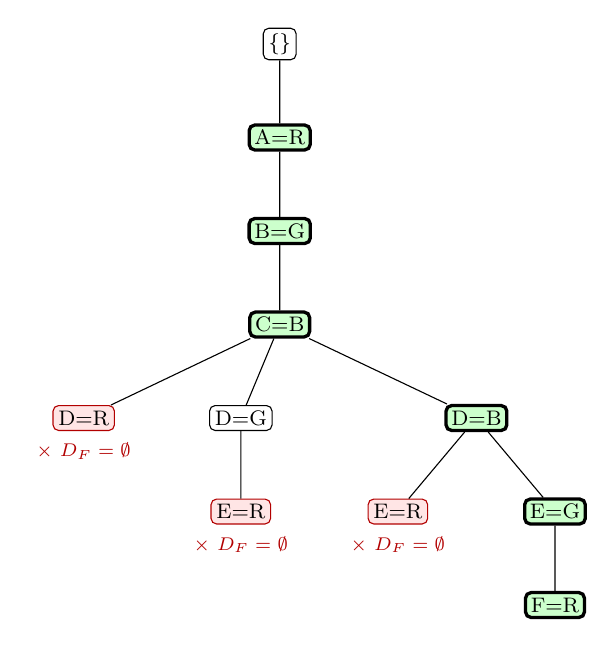
\begin{tikzpicture}[scale=0.95, every node/.style={transform shape}, bn/.style={draw, rounded corners=2pt, font=\footnotesize, inner sep=2pt}]
\node[bn] (b1) at (2.62,0.00) {$\{\}$};
\node[bn, fill=green!20, very thick] (b2) at (2.62,-1.25) {A$=$R};
\node[bn, fill=green!20, very thick] (b3) at (2.62,-2.50) {B$=$G};
\node[bn, fill=green!20, very thick] (b4) at (2.62,-3.75) {C$=$B};
\node[bn, fill=red!10, draw=red!70!black] (b5) at (0.00,-5.00) {D$=$R};
\node[font=\scriptsize, text=red!70!black, below=1pt of b5] {$\times$ $D_{F}=\emptyset$};
\draw (b4) -- (b5);
\node[bn] (b6) at (2.10,-5.00) {D$=$G};
\node[bn, fill=red!10, draw=red!70!black] (b7) at (2.10,-6.25) {E$=$R};
\node[font=\scriptsize, text=red!70!black, below=1pt of b7] {$\times$ $D_{F}=\emptyset$};
\draw (b6) -- (b7);
\draw (b4) -- (b6);
\node[bn, fill=green!20, very thick] (b8) at (5.25,-5.00) {D$=$B};
\node[bn, fill=red!10, draw=red!70!black] (b9) at (4.20,-6.25) {E$=$R};
\node[font=\scriptsize, text=red!70!black, below=1pt of b9] {$\times$ $D_{F}=\emptyset$};
\draw (b8) -- (b9);
\node[bn, fill=green!20, very thick] (b10) at (6.30,-6.25) {E$=$G};
\node[bn, fill=green!20, very thick] (b11) at (6.30,-7.50) {F$=$R};
\draw (b10) -- (b11);
\draw (b8) -- (b10);
\draw (b4) -- (b8);
\draw (b3) -- (b4);
\draw (b2) -- (b3);
\draw (b1) -- (b2);
\end{tikzpicture}
\end{adjustbox}
\end{center}Forward checking empties a domain 3 times and the search backtracks 4 times (solution A=R, B=G, C=B, D=B, E=G, F=R). After $D=G$, FC leaves $E=\{R\}$ and $F=\{R\}$ although E and F are adjacent: FC does not check arcs between unassigned variables, while arc consistency would.
\end{solbox}
\question{9}Variables $A,B,C\in\{1,\dots,6\}$ with the constraints $A=2B$, $B+C=7$ and $A<C$.
\subq{(a)}Run AC-3 starting from the queue $A\to B,\ B\to A,\ B\to C,\ C\to B,\ A\to C,\ C\to A$ (pop from the front; when $D_i$ shrinks, append every arc $X_k\to X_i$, $k\neq j$, not already queued). Show every revision.
\begin{solbox}
\begin{center}\small\begin{tabular}{c c c l p{5cm}}\toprule
\# & Arc popped & Removed from tail & New domain & Arcs appended to queue \\ \midrule
1 & $A \to B$ & 1, 3, 5 & $D_{A}=\{2,4,6\}$ & -- \\
2 & $B \to A$ & 4, 5, 6 & $D_{B}=\{1,2,3\}$ & -- \\
3 & $B \to C$ & -- &  & -- \\
4 & $C \to B$ & 1, 2, 3 & $D_{C}=\{4,5,6\}$ & -- \\
5 & $A \to C$ & 6 & $D_{A}=\{2,4\}$ & $B\to A$ \\
6 & $C \to A$ & -- &  & -- \\
7 & $B \to A$ & 3 & $D_{B}=\{1,2\}$ & $C\to B$ \\
8 & $C \to B$ & 4 & $D_{C}=\{5,6\}$ & $A\to C$ \\
9 & $A \to C$ & -- &  & -- \\
\bottomrule\end{tabular}\end{center}
\end{solbox}
\subq{(b)}Cross out the eliminated values, and give all solutions.\begin{center}\small\begin{tabular}{|l|c|c|c|}\hline Variables & \textbf{A} & \textbf{B} & \textbf{C}\\ \hline Domains & 1\ 2\ 3\ 4\ 5\ 6 & 1\ 2\ 3\ 4\ 5\ 6 & 1\ 2\ 3\ 4\ 5\ 6\\ \hline\end{tabular}\end{center}
\begin{solbox}
\begin{center}\small\begin{tabular}{|l|c|c|c|}\hline Variables & \textbf{A} & \textbf{B} & \textbf{C}\\ \hline Domains & \textcolor{red!70!black}{\sout{1}}\ 2\ \textcolor{red!70!black}{\sout{3}}\ 4\ \textcolor{red!70!black}{\sout{5}}\ \textcolor{red!70!black}{\sout{6}} & 1\ 2\ \textcolor{red!70!black}{\sout{3}}\ \textcolor{red!70!black}{\sout{4}}\ \textcolor{red!70!black}{\sout{5}}\ \textcolor{red!70!black}{\sout{6}} & \textcolor{red!70!black}{\sout{1}}\ \textcolor{red!70!black}{\sout{2}}\ \textcolor{red!70!black}{\sout{3}}\ \textcolor{red!70!black}{\sout{4}}\ 5\ 6\\ \hline\end{tabular}\end{center}Solutions $(A,B,C)$: $(2,1,6)$, $(4,2,5)$.
\end{solbox}
\question{10}Answer the following questions briefly.
\subq{(a)}What is a rational agent? Using the lecture's examples (fingers on a hot stove; crossing at a crosswalk), distinguish a reflex action from an intelligent action. Can a reflex action be rational?
\begin{solbox}
A rational agent acts to achieve the best outcome, or the best expected outcome under uncertainty. A reflex action is immediate, without deliberation (withdrawing the fingers); an intelligent action results from reasoning or learning (crossing at the crosswalk). A reflex action can be rational or not; intelligent actions are usually rational.
\end{solbox}
\subq{(b)}What is abstraction in problem formulation? When is an abstraction valid and when is it useful? Illustrate with route finding in Romania.
\begin{solbox}
Removing detail from the representation (the state is just the current city; weather, traffic, companions are ignored). Valid: every abstract solution can be turned into a real one; useful: each abstract action (drive Arad$\to$Sibiu) is easier than the original problem.
\end{solbox}
\subq{(c)}For 8-queens, compare the naive incremental formulation, the improved incremental formulation and the complete-state formulation used by hill climbing (size of the space / number of successors).
\begin{solbox}
Naive (add a queen to any empty square): $64\cdot63\cdots57\approx1.8\times10^{14}$ sequences. Improved (one queen per column, leftmost empty column, non-attacked squares only): 2{,}057 states. Complete-state (8 queens, one per column, move a queen in its column): $8\times7=56$ successors per state.
\end{solbox}
\subq{(d)}List the four steps of an MCTS iteration and explain the difference between the tree policy and the default policy.
\begin{solbox}
Selection, Expansion, Simulation (rollout), Backpropagation. The tree policy (e.g.\ UCB1) chooses nodes inside the tree; the default policy plays the rollout outside the tree (uniformly random and fast by default).
\end{solbox}
\question{11}True or false?
For each statement, circle \textbf{T} or \textbf{F} and justify your answer in one or two sentences (an answer without a correct justification earns no credit).
\subq{1.}Tree-search DFS without any cycle checking is complete on every finite state space. \hfill \textbf{T \quad F}
\begin{solbox}
\F. With cycles (e.g.\ two states linked both ways) it can loop forever; checking the current path fixes this.
\end{solbox}
\subq{2.}Uniform-cost search is complete if every action cost is at least some $\epsilon>0$. \hfill \textbf{T \quad F}
\begin{solbox}
\T. Then any path cost grows without bound with its length, so UCS cannot get stuck on an infinite path of tiny costs.
\end{solbox}
\subq{3.}Tree-search DFS needs only $O(bm)$ memory. \hfill \textbf{T \quad F}
\begin{solbox}
\T. It stores one path and the unexpanded siblings along it.
\end{solbox}
\subq{4.}Greedy best-first graph search is complete in finite state spaces. \hfill \textbf{T \quad F}
\begin{solbox}
\T. It never re-expands a state, so it eventually exhausts a finite space.
\end{solbox}
\subq{5.}Weighted A* ($f=g+W\cdot h$, $W>1$) always returns an optimal path when $h$ is admissible. \hfill \textbf{T \quad F}
\begin{solbox}
\F. $W\cdot h$ may overestimate; weighted A* trades optimality for speed.
\end{solbox}
\subq{6.}Minimax has time complexity $O(b^m)$ and space complexity $O(bm)$. \hfill \textbf{T \quad F}
\begin{solbox}
\T. It is a complete depth-first exploration of the game tree.
\end{solbox}
\subq{7.}An order-preserving transformation of the leaf values never changes the move chosen by expectimax. \hfill \textbf{T \quad F}
\begin{solbox}
\F. True for minimax, not for expectimax (see Question 6).
\end{solbox}
\subq{8.}The robust child of the MCTS root is the child with the highest average reward. \hfill \textbf{T \quad F}
\begin{solbox}
\F. Robust = most visited; highest average = max child.
\end{solbox}
\subq{9.}AC-3 runs in $O(cd^3)$ in the worst case. \hfill \textbf{T \quad F}
\begin{solbox}
\T. Each arc is re-queued at most $d$ times and each revision costs $O(d^2)$.
\end{solbox}
\subq{10.}Forward checking makes the neighbours of the just-assigned variable consistent with it, but does not look further ahead. \hfill \textbf{T \quad F}
\begin{solbox}
\T. That is exactly FC; MAC continues propagating with AC-3.
\end{solbox}
\end{document}